%%  Using official ACM format
%% Do not edit unless you really know what you are doing.
\documentclass{acm_proc_article-sp}
% % % % % % % % % % % % % % % % % % % % % % % % % % % % % % % % % % % %
% Definitions
% % % % % % % % % % % % % % % % % % % % % % % % % % % % % % % % % % % %
\def\firstUserCase{1} % set to 1 to build user cases on their own pages
% % % % % % % % % % % % % % % % % % % % % % % % % % % % % % % % % % % %
%\usepackage[T1]{fontenc}
%\usepackage[latin9]{inputenc}
%\usepackage{fancyhdr}
%\pagestyle{fancy}
\usepackage{graphicx}
%\usepackage{babel}
\usepackage[pdftitle={Optimistic Control for a Critical System},%
		hidelinks,colorlinks=true, linkcolor=black, citecolor=cyan, filecolor=green, urlcolor=blue]{hyperref}
\usepackage{mathtools}
\usepackage{amssymb}

% % % % % % % % % % % % % % % % % % % % % % % % % %
% Aconyms for SyncFree project.
%
% Author: Amadeo Asco
% Last updated: 24 July 2014
% % % % % % % % % % % % % % % % % % % % % % % % % %
% The acronym package helps you manage acronyms and acronym lists in your documents, http://www.mackichan.com/index.html?techtalk/456.htm~mainFrame
% for the glossary to show up in Table of Contents you need to additionally add toc option
\usepackage[toc,nonumberlist]{glossaries}
%\showthe\hsize% interrupts latex and shows value of \hsize
\setlength{\glsdescwidth}{0.82\hsize}%
% to remove extra line between groups
\renewcommand{\glsgroupskip}{}
% To get rid of the full stop after the description in the glossary
\renewcommand{\glspostdescription}{}
\makeglossaries

% Start definitions ---------------------------
% Add all of the definitions for the abbreviations
\newacronym{2i}{2i}{Secondary Indexing}
\newacronym{2pset}{2P-Set}{Two-Phase Set}
\newacronym{acid}{ACID}{Atomicity, Consistency, Isolation, Durability}
\newacronym{b2b}{B2B}{Business to Business}
\newacronym{base}{BASE}{basically available, soft state, eventual consistency}
\newacronym{cci}{CCI}{Causality, Convergence and Intention}
\newacronym{cmrdt}{CmRDT}{Op-based Convergent Replicated Data Type}
\newacronym{cprdt}{CPRDT}{Conflict-free Partially Replicated Data Type}
\newacronym{crdt}{CRDT}{Conflict-free Replicated Data Type}
\newacronym{cqrs}{CQRS}{Command Query Responsibility Segregation}
\newacronym{cvrdt}{CvRDT}{State-based Convergent Replicated Data Type}
\newacronym{dc}{DC}{Data Centre}
\newacronym{ec}{EC}{Eventual Consistency}
\newacronym{ga}{GA}{Genetic Algorithm}
\newacronym{gset}{G-set}{State-based increment-only Counter}
\newacronym{gp}{GP}{General Practitioner}
\newacronym{ha}{HA}{High Availability}
\newacronym{id}{ID}{identifier}
\newacronym{lww}{LWW}{Last-Writer-Wins}
\newacronym{lwwr}{LWW-Register}{Last-Writer-Wins Register}
\newacronym{mdc}{MDC}{Multi Data Centre}
\newacronym{mv}{MV}{Multi-Valued}
\newacronym{mvr}{MV-Register}{Multi-Valued Register}
\newacronym{orset}{OR-set}{Observed-Removed Set}
\newacronym{rdbms}{RDBMS}{Relational Database Management System}
\newacronym{rga}{RGA}{Replicated Growing Array}
\newacronym{rest}{REST}{Representational State Transfer}
\newacronym{rpc}{RPC}{Remote Procedure Call}
\newacronym{cap}{CAP}{Consistency, Availability and Partition tolerance}
\newacronym{sec}{SEC}{Strong Eventual Consistency}
\newacronym{ttl}{TTL}{Time To Live}
\newacronym{uset}{U-Set}{Two-Phase Set with unique elements}
\newacronym{wp1}{WP1}{Work Package 1}
\newacronym{wp2}{WP2}{Work Package 2}
\newacronym{wp3}{WP3}{Work Package 3}
\newacronym{wp4}{WP4}{Work Package 4}
\newacronym{wp5}{WP5}{Work Package 5}
% end abbreviations ---------------------------

%\ifnum\showDefinitions=1
% Add all of the definitions
%\newglossaryentry{bwd}{name={box-and-whisker diagram}, text={box-and-whisker diagram}, first={box-and-whisker diagram},
%    description={\parbox{10.6cm}{\medskip The bottom and top of the box are the 25th and 75th percentile (the lower and upper quartiles, respectively), and the band near the middle of the box is the median, whereas the dot represent the mean. The ends of the whiskers represent the minimum and maximum of all of the data.\medskip}}}
% end definitions -----------------------------
%\fi

\glsdisablehyper


\begin{document}

\title{Formal Mathematical Requirements\\(work in progress)}
%
% You need the command \numberofauthors to handle the 'placement and alignment' of the authors beneath the title.
%
% For aesthetic reasons, we recommend 'three authors at a time', i.e. three 'name/affiliation blocks' be placed beneath the title.
%
% NOTE: You are NOT restricted in how many 'rows' of "name/affiliations" may appear. We just ask that you restrict the number of 'columns' to three.
%
% Because of the available 'opening page real-estate' we ask you to refrain from putting more than six authors (two rows with three columns) beneath the article title.
% More than six makes the first-page appear very cluttered indeed.
%
% Use the \alignauthor commands to handle the names and affiliations for an 'aesthetic maximum' of six authors.
% Add names, affiliations, addresses for the seventh etc. author(s) as the argument for the
% \additionalauthors command.
% These 'additional authors' will be output/set for you without further effort on your part as the last section in the body of your article BEFORE References or any Appendices.

\numberofauthors{2} %  in this sample file, there are a *total*
% of EIGHT authors. SIX appear on the 'first-page' (for formatting reasons) and the remaining two appear in the \additionalauthors section.
%
\author{
% 1st. author
	\alignauthor
	Tom Benedictu\\
	\affaddr{Trifork Leeds}\\
	\email{tom@trifork.com}
% 2nd. author
	\alignauthor
	Amadeo Asco\\
	\affaddr{Trifork Leeds}\\
	\email{aas@trifork.com}
}

% There's nothing stopping you putting the seventh, eighth, etc. author on the opening page (as the 'third row') but we ask, for aesthetic reasons that you place these 'additional authors' in the \additional authors block, viz.
%\additionalauthors{Additional authors: John Smith (The Th{\o}rv{\"a}ld Group,
%	email: {\texttt{jsmith@affiliation.org}}) and Julius P.~Kumquat
%	(The Kumquat Consortium, email: {\texttt{jpkumquat@consortium.net}}).}
\date{28 July 2014}

\maketitle
\begin{abstract}
Building reliable distributed systems, given the CAP theorem where partitioning must always be considered, relays in the trade-offs between consistency and availability. \glspl{crdt} define replicated data types with mathematical properties that ensure absence of conflict and confer them \gls{sec}, a form of \gls{ec} which it is a technique of compromise.  Consistency is a property of the data, not the datastore, given that the rules to decide how to synchronise are business decisions. \glspl{crdt} have been created to ensure that we have a computer model for handling data which accommodates data's nature in a world of vast communication and no definite central place of storage. Using an \gls{rdbms} for these type of systems can result in systems where a large amount of the processing is required to circumnavigate the shortcomings of a model that is not fit for purpose. A significant project for mediating this dilemma is \href{https://syncfree.lip6.fr}{SyncFree}.

%For SyncFree we are gathering requirements from a range of large-scale distributed applications which all have been implemented recently or are in the process of being implemented.

%The goal of SyncFree is to enable large-scale distributed applications without global synchronization, by exploiting the recent concept of \glspl{crdt}. \glspl{crdt} allow non-synchronized concurrent updates, yet ensure data consistency. This revolutionary approach maximizes responsiveness and availability; it enables locating data near its users, in decentralized clouds.

%For reference and later validation of the developed tools we are gathering requirements from a number of representative applications. This is the work carried out in \gls{wp1}. \gls{wp1} is divided into two succeeding parts, where the first has just been completed. The first is to describe the requirements in natural language and the second is to transform this description into a formal mathematical language.

This article provides a brief presentation of the natural language requirements, which shows the special nature of the paradigm shift forcing large-scale distributed applications away from \gls{rdbms}.
\newpage
\end{abstract}

% A category with the (minimum) three required fields
%\category{H.4}{Information Systems Applications}{Miscellaneous}
%A category including the fourth, optional field follows...
%\category{D.2.8}{Software Engineering}{Metrics}[complexity measures, performance measures]
%\category{D.2.1}{Software Engineering}{Requirements/Specifications}[user cases]
\category{H.2.4}{Systems}[concurrency, distributed databases]

\terms{Documentation, Reliability}

\keywords{CRDTs, Use cases, SyncFree} % NOT required for Proceedings


\section{Introduction}
\gls{ec} is one key element in the concept for a contemporary replicated database, presented in \cite{Shapiro2009a}, \cite{Saito2005a}, that takes into account the CAP theorem \cite{Abadi2012consistency, Gilbert2002a, Brewer2000cap} . In fact, the database comprises data traversing the cloud together with data residing on devices, not yet if ever, going to move to another storage which is here referred to as the edge of the network. \gls{acid} are the classic requirements for a database. We want to retain these although we realise that they may be relaxed in some areas and they should be avoided in other areas. Atomicity indicates that either the entire transaction can be carried out or it will be rolled back to the state before it was even started. In a large-scale distributed application this criteria cannot be accommodated in a reliable fashion as it results in deadlocks. Consistency cannot be guaranteed as part of the atomic transaction. We are trusting \gls{ec}, which has been a prolific topic of research \cite{shapiro11comprehensive}, \cite{Vogels2009a}, \cite{Saito2005a}, \cite{Baquero1997a}, and provisioning mechanisms for detecting persistent inconsistencies. \gls{ec} is a weaker data consistency which will require a complex background algorithm for reconciling conflicting updates \cite{Terry1995a}. \glspl{crdt} have been designed to solve the need for reconciliation by using \gls{sec} \cite{shapiro11conflictfree}, without the need of complex conflict resolution, roll-backs, or consensus. Also composites of \glspl{crdt} present the same properties, \cite{Deftu2013a}, \cite{shapiro11comprehensive}.

\section{Use Cases}
Three use cases has been identified from Rovio representing significant issues and difficulties of extreme-scale sharing and consistency within online and mobile large scale entertainment application. Further we have three distinct use cases from Trifork each representing their own application domain and each posing issues that requires \glspl{crdt}.

We are here providing an overview to illustrate the nature of the requirements we are faced with in large-scale distributed applications without global synchronisation.

The general constants and variables that applied to all the following use cases are presented in Table \ref{tab:general_definitions}.
\begin{table}[!ht]
	\begin{tabular}{|p{1cm}|p{5.6cm}|r| }
		\hline
		\multicolumn{1}{|c|}{Name} & \multicolumn{1}{c|}{Description} & \multicolumn{1}{c|}{Type} \\
		\hline
		\hline
		$DC$ & It is the set of all \glspl{dc}. $d$ identifies one of the \glspl{dc}, $d \in DC$, where $|DC|$ is the number of \glspl{dc}. & $\mathbb{Z}_{+} $\\
		\hline
		$DV$ & It is the set of devices. $dv$ represents one of those devices, $dv \in DV$, where $|DV|$ is the number of devices. & $\mathbb{Z}_{+}$ \\
		\hline
		$Nodes$ & It is the set of nodes. $n$ represents one of those nodes, $n \in Node$, where $|Nodes|$ is the number of nodes in a \gls{dc}. & $\mathbb{Z}_{+}$ \\
		\hline
		$Clients$ & it is the set of clients and $c$ represents a client in the system, $c \in Clients$, where $|Clients|$ is the total number of clients. & $\mathbb{Z}_{+}$ \\
		\hline
	\end{tabular}

	\caption{General definitions.}
	\label{tab:general_definitions}
\end{table}

\section{Entertainment Applications}
Rovio, being one of the leaders in online and mobile entertainment, has provided three unique use cases from their current applications. These use cases are also relevant for many other possible application domains and are as such highly relevant for establishing the requirements for \glspl{crdt}.

%%%%%%%%%%%%%%%%%%%%%%%%%%%%%%%%%%%%%%%%%
% Use cases
%%%%%%%%%%%%%%%%%%%%%%%%%%%%%%%%%%%%%%%%%
\ifnum\firstUserCase=1
	\newpage
\fi
\subsection{Advertisement Counter}
Advertising platforms need to accurately record impressions and clicks, in order to analyse advertising data. They use distributed counters, which are challenging to implement in a dynamic, fault-prone environment. \gls{crdt} counters are a promising solution; the challenge is to scale to an extreme numbers of users.

Rovio's Ads service keeps track of impressions and clicks for ads per campaign/ad/country. Typically these counts have some upper bounds after which the ad should not be shown any more. The upper bound may consist of the sum of several counters (e.g show the same ad 50,000 times in the US, 10,000 times in the UK and 100,000 times in total), so it is not really feasible to enforce the upper bound on the data storage layer.

The main use for the tracking data is to control the rate of ads shown to the users. The campaign capacity should be spread evenly over the duration of the campaign instead of showing all the impressions during the first hour of the campaign. Therefore, the data must be updated in real time although a good estimate is normally enough. 


\subsubsection{Current Implementation}
The system maybe represented by the various constants and variables that follow, Table \ref{tab:ads_constants_variables}.
\begin{table}[!ht]
	\begin{tabular}{|p{0.7cm}|p{5.8cm}|r| }
		\hline
			\multicolumn{1}{|c|}{Name} & \multicolumn{1}{c|}{Description} & \multicolumn{1}{c|}{Type} \\
		\hline
		\hline
%			$DC$ & It is the set of all \glspl{dc}. $d$ identifies one of the \glspl{dc}, $d \in \{1,\dots, |DC|\}$. & $\mathbb{Z}_{+} $\\
%		\hline
			$AD$ & It is the set of all advertisement-campaigns. $a$ identify one of the ads, $a \in AD$, where $|AD|$ is the number of ads. & $\mathbb{Z}_{+}$ \\
		\hline
%			$DV$ & It is the set of devices. $dv$ represents one of those devices, $dv \in \{1,\dots, |DV|\}$. & $\mathbb{Z}_{+}$ \\
%		\hline
%			$Nodes$ & It is the set of nodes. $n$ represents one of those nodes, $n \in \{1,\dots, |Nodes|\}$. & $\mathbb{Z}_{+}$ \\
%		\hline
	\end{tabular}
	\vspace{.1cm}

	\begin{tabular}{|p{7cm}|p{.2cm}| }
		\hline
			Name/Description & \multicolumn{1}{c|}{Type} \\
		\hline
		\hline
			$T_{a}, T^{start}_{a}, T^{end}_{a}$ & $\mathbb{R}_{+}$ \\
		\hline
			 \multicolumn{2}{|p{7.1cm}|}{$T_{a}$ is the duration of the campaign for ad $a$.
			$T^{start}_{a}$ represents the beginning of the campaign and $T^{end}_{a}$ the end, with $T_{a}= T^{start}_{a} - T^{end}_{a}$.}\\
		\hline
		\hline
			$maxTotalViews(a)$ & $\mathbb{Z}_{+}$ \\
		\hline
			\multicolumn{2}{|p{7.1cm}|}{It is the maximum total number of times the ad $a$ should be shown.} \\
		\hline
		\hline
			$maxTotalViewsPerDC(a, d)$ & $\mathbb{Z}_{+}$ \\
		\hline
			 \multicolumn{2}{|p{7.1cm}|}{It is the total number of times the ad $a$ should be shown by \gls{dc} $d$.} \\
		\hline
		\hline
			$maxViewsPerDevice(a)$ & $\mathbb{Z}_{+}$ \\
		\hline
			\multicolumn{2}{|p{7.1cm}|}{It represents the maximum number of times the ad $a$ should be presented on a device.} \\
		\hline
		\hline
			$viewsPerDevice(a, dv)$ & $\mathbb{Z}_{+}$ \\
		\hline
			\multicolumn{2}{|p{7.1cm}|}{It is the number of times the ad $a$ has been shown on the device $g$. $h(t)_{ag}$ is the same than $h_{ag}$.} \\
		\hline
		\hline
			$verifiedViews(a, n, q)$ & $\mathbb{Z}_{+}$ \\
		\hline
			\multicolumn{2}{|p{7.1cm}|}{It is the verified number of times an ad $a$ has been shown by node $q$ as the node $n$ report it, $n, q \in \{1,\dots, |Nodes|\}$.} \\
		\hline
		\hline
			$averageViews(a)$ & $\mathbb{Z}_{+}$ \\
		\hline
			\multicolumn{2}{|p{8.1cm}|}{It is the average number of times ad $a$ is shown. The workload is equally spread between all the nodes, $\frac{averageViews(a)}{|Nodes|}$.} \\
		\hline
	\end{tabular}

	\caption{Ad Counters Constants and Variables.}
	\label{tab:ads_constants_variables}
\end{table}

Equality \ref{eq:ad_spread} states that the total maximum number of times an ad should be presented in each \gls{dc} is equal to  the maximum total number of times that ad should be shown in the campaign, and Inequality \ref{eq:total_device_ads} states that the ad $a$ must be shown on any device only a maximum number of times of $maxTotalViews(a)$. The total number of times that ad $a$ has been shown on completion of the campaign is expressed by Equation \ref{eq:real_total_ads}. The goal of the system is to minimise $\Delta_{a}$, $\Delta_{a} \in \mathbb{N}_{0}$.
\begin{equation} \label{eq:ad_spread}
	maxTotalViews(a) = \sum_{d \in DC} maxTotalViewsPerDC(a, d)
\end{equation}
\begin{equation} \label{eq:total_device_ads}
	maxViewsPerDevice(a) \ge viewsPerDevice(a, dv)
\end{equation}
\begin{multline} \label{eq:real_total_ads}
	maxTotalViews(a) = \sum_{dv \in DV} viewsPerDevice(a, dv) + \Delta_{a}\\ \forall ~  t \ge T^{end}_{a}
\end{multline}

The Ads service runs on multiple service nodes, so in order to avoid write conflicts each of those nodes has its own document for the impression and click counters in Riak. This is already a simplified implementation of the counter \gls{crdt}. The true value of the counter can be obtained by calculating the sum of all counters manually.

Even if the current solution works, it is neither very elegant nor easy to maintain. The \gls{crdt} counters will provide a more efficient solution for updating the counters. The ad system does not need a strict limit for the counter and we can implement an optimistic solution: if the counter value is less than the limit then show the ad and increase the counter. This may result in showing the ad too many times, but it is \textquotedbl{}close enough\textquotedbl{}. Client applications running on different kinds of devices (mobile phones, tablets, etc.) connect to the Ads service in order to determine which ads to show to their users. The same ad should not be shown on the same device any more than 3 times a day ($maxViewsPerDevice(a, dv) = 3$), so the Ads service keeps track of on which device has been shown which ad and when. This data is currently stored in one document that contains information on the ads shown on a device during the last couple of days (basically which ad has been shown and when). It might be possible to utilise \glspl{crdt} in this document.
%, but the current implementation has no major issues, either.

In a \gls{dc} each server node has its own cache representing the counters. The cache could be dropped theoretically, but in practice it will be needed. The counters get synced between the life statistics nodes via Riak. Each counter will have some copies, e.g. three, on the database meaning the value is formed based on those copies. The average number of times, ad $a$ is shown, is $averageViews(a)$  for an interval of time, so the estimated number of times the ad $a$ has been shown is represented by Equation \ref{eq:dc_counter} as seen by node $n$, note that only one \gls{dc} is currently used. Also the verified number of times an ad has been shown, $ verifiedViews(a, n)$, is the number of times node $n$ reported to have shown the ad $a$ in the last synchronisation at previous period of time.
\begin{multline} \label{eq:dc_counter}
	views(a, n) = \sum_{q \in Nodes}  verifiedViews(a, n, q)\\ + averageViews(a)
\end{multline}

The sum of all the times an ad $a$ has been seen corresponds to the real number of times the ad $a$ has been shown by the system, as shown by Equation \ref{eq:real_dc_counter}. The total number os times the ad $a$ has been seen at any time, $views(a, n)$, as seen by a node $n$ may be less or equal to the real total number of times the ad $a$ has been shown, $views(a)$, as shown by Inequality \ref{eq:compare_dc_counters}. This inequality should be eventually (after last synchronisation) an equality.
\begin{equation} \label{eq:real_dc_counter}
	views(a) = \sum_{n \in Nodes}  verifiedViews(a, n, n)
\end{equation}
\begin{equation} \label{eq:compare_dc_counters}
	views(a) \ge views(a, n)
\end{equation}

Also the numbers of times an ad $a$ has been shown after the ad-campaign has concluded must be the same irrespective of the node reporting it, as shown by Equation \ref{eq:dc_counter_per_node}.
\begin{multline} \label{eq:dc_counter_per_node}
	views(a) = views(a, n) = views(a, m)\\ \forall ~ n, m \in \{1,\dots, |Nodes|\}, t \ge T^{end}_{a} + \Delta t
\end{multline}

The life statistics nodes serve the entire state of all campaigns. They hold a cache for the data and keep it in sync via Riak. There is a local estimation in place between the nodes synchronisation since the data is not synced on every update they get from the ad servers.


\subsubsection{Multiple Data Centres}
The campaign counter could also be split between the different \glspl{dc} in each country which will improve the accuracy of the counter, Figure \ref{fig:ads_countert_}. At each \gls{dc} a part of the overall counter would be assigned to each \gls{dc}, which will only be able to service this number of times the specific ad. The changes to the ad counters are replicated in the other \glspl{dc} at different intervals.
\begin{figure*}[ht!]
	\centering
	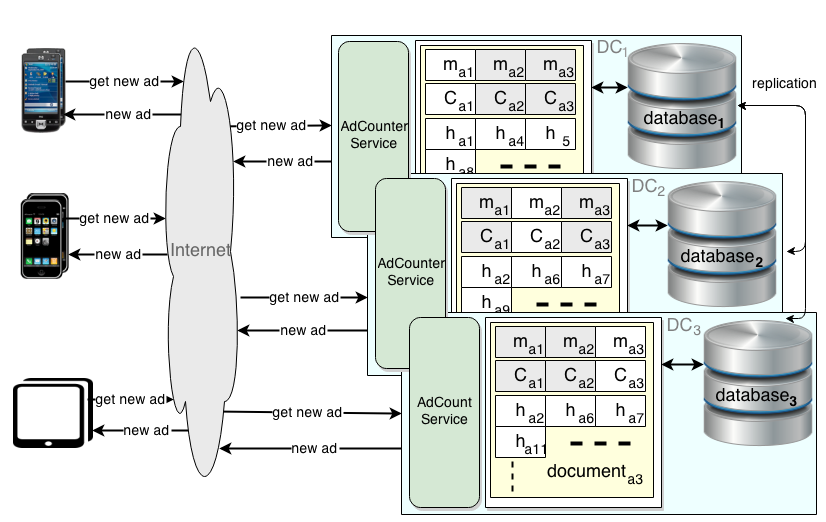
\includegraphics[width=1\linewidth]{figures/AdsServiceSpread2DCs.png}

	\caption{Overview for the distribution of counters with three \glspl{dc}, $|DC| = 3$, $m_{ad} \equiv targetMaxViews(a, d)$, $C_{ad} \equiv maxViewsPerDevice(a)$ and $h(a, g) \equiv views(a, d, g)$.}
	\label{fig:ads_countert_}
\end{figure*}

The distribution of the counter could be based on different criterion, e.g. population size covered by each \gls{dc}, existing statistics from previous campaigns or studies, costumer preferences, intention of the campaign like the increase in the market share in an already established part of the territory or entering a new area to extend the territory covered.

It may be decided that when a device serviced by a \gls{dc} changes to be serviced by another \gls{dc}, e.g. by changing location, then its counter is now know by the new servicing \gls{dc}, potentially showing those ads already seen again, otherwise the device counter needs to be replicated between \glspl{dc}, but not necessarily to all \glspl{dc}.

The extra constants required for multiple \glspl{dc} are presented below, Table \ref{tab:ads_extra_constants_variables}.
\begin{table}[!ht]
	\begin{tabular}{|p{6.5cm}|p{.2cm}|}
		\hline
			Name/Description & \multicolumn{1}{c|}{Type} \\
		\hline
		\hline
			$Nodes_{d}$ & $\mathbb{Z}_{+}$ \\
		\hline
			\multicolumn{2}{|p{8.1cm}|}{It is the set of nodes in \gls{dc} $d$. $n$ represents one of those nodes, $n \in \{1,\dots, |Nodes_{d}|\}$.} \\
		\hline
		\hline
			$averageViews(a, d)$ & $\mathbb{Z}_{+}$ \\
		\hline
			\multicolumn{2}{|p{8.1cm}|}{It is the average number of times ad $a$ is shown for a given time interval by \gls{dc} $d$. The workload is equally spread between all the nodes in the same \gls{dc}, $\frac{averageViews(a, d)}{|Nodes_{d}|}$.} \\
		\hline
		\hline
			$verifiedViews(a, d, n)$ & $\mathbb{Z}_{+}$ \\
		\hline
			\multicolumn{2}{|p{8.1cm}|}{It is the verified number of times an ad $a$ has been shown by node $n$ in \gls{dc} $d$ as the node $n$ reported to have shown the ad $a$ in the last synchronisation at previous period of time.} \\
		\hline
		\hline
			$targerMaxViews(a, d)$ & $\mathbb{Z}_{+}$ \\
		\hline
			\multicolumn{2}{|p{8.1cm}|}{It is the maximum number of times the ad $a$ should be shown by \gls{dc} $d$. This may as well be used to restrict the locations (represented by $L$), e.g. country an ad is shown. \glspl{dc} outside these locations will not show the ad so $targerMaxViews(a, d) = 0 ~ \forall ~ a \not\in L$. Also the replication will only be necessary between the \glspl{dc} with $targerMaxViews(a, d) > 0$.} \\
		\hline
		\hline
			$views(a, d)$ & $\mathbb{N}_{0}$ \\
		\hline
			\multicolumn{2}{|p{8.1cm}|}{It is the total number of times the ad $a$ has been shown on devices by \gls{dc} $d$ from the beginning of the campaign, $T^{start}_{a}$, to time $t$.} \\
		\hline
		\hline
			$totalViews(a)$ & $\mathbb{Z}_{+}$ \\
		\hline
			\multicolumn{2}{|p{8.1cm}|}{It is the overall total number of times the ad $a$ has been shown from the beginning of the campaign, $T^{start}_{a}$, to time t.} \\
		\hline
	\end{tabular}

	\caption{Ad Counters extra Constants and Variable.}
	\label{tab:ads_extra_constants_variables}
\end{table}

The model needs to be extended by the following expressions:
\begin{equation} \label{eq:dcs_counter_limit}
	targetMaxViews(a, d) \ge views(a, d)
\end{equation}
\begin{equation} \label{eq:dcs_counter_start}
	views(a, d) = 0 ~ \forall ~ t \le T^{start}_{a}
\end{equation}
\begin{equation} \label{eq:dcs_counter_final}
	targetMaxViews(a, d) =  views(a, d) ~ \forall ~ t \ge T^{end}_{a}
\end{equation}
\begin{equation} \label{eq:total_ads}
	totalMaxView(a)  = \sum_{d \in DC} targetMaxViews(a, d)
\end{equation}
\begin{equation} \label{eq:total_ads_at_time_t}
	totalViews(a) =  \sum_{d \in DC} views(a, d)
\end{equation}
Inequality \ref{eq:dcs_counter_limit} states that the counter $views(a, d)$ always has a limit which it is the maximum number of times the ad $d$ must be shown by \gls{dc} $d$, whereas at the beginning of the campaign no ads has been shown as stated by Equation \ref{eq:dcs_counter_start}, and once the campaign has finish the total number of times an ad has been shown by each \gls{dc} is the same than the maximum allowed as expressed by Equation \ref{eq:dcs_counter_final}. Equation \ref{eq:total_ads} states that the ads are distributed through out all the \glspl{dc}. Equation \ref{eq:total_ads_at_time_t} states that the overall total number of times an ad $a$ has been shown is equal to the sum of the number of times the ad $a$ has been shown by each \gls{dc}.

\begin{equation} \label{eq:total_ads2}
	maxTotalViews(a) \ge \sum_{d \in DC} totalViews(a, d)
\end{equation}
\begin{equation} \label{eq:total_ads3}
	maxTotalViews(a) = totalViews(a) + \Delta_{a} ~ \forall ~ t \ge T^{end}_{a}
\end{equation}
Inequality \ref{eq:total_ads2} gives the total limit for all the $totalViews(a, d)$ which can be obtained from Inequality \ref{eq:dcs_counter_limit} and Equation \ref{eq:total_ads}, whereas Equation \ref{eq:total_ads3} shows that the total number of times ad $a$ has been shown, once the campaign has concluded $t \ge T$, is equal to the total number ad $a$ should has been shown.

Also Equation \ref{eq:dc_counter} can be generalised for many \glspl{dc} as shown in Equation \ref{eq:dc_total_counter}.
\begin{multline} \label{eq:dc_total_counter}
	views(a, d) = \sum_{n \in Nodes_{d}}  verifiedViews(a, d, n) +\\ averageViews(a, d)
\end{multline}

There is the possibility that a device in the border between two \glspl{dc}, where the ad is run, receives more than its limit if the two \glspl{dc} are out of sync for that device.

To have into account the state of the data in each of the \glspl{dc} the previous definitions are extended and some new introduced below, Table \ref{tab:ads_entended_constants_variables}.
\begin{table}[!ht]
	\begin{tabular}{|p{6.5cm}|p{.2cm}| }
		\hline
			Name/Description & \multicolumn{1}{c|}{Type} \\
		\hline
		\hline
			 $views(a, d, q)$ & $\mathbb{Z}_{+}$ \\
		\hline
			\multicolumn{2}{|p{8.1cm}|}{It is the total number of times the ad $a$ has been shown on devices by \gls{dc} $d$ from the beginning of the campaign to time $t$ as it is seen by \gls{dc} $q$, $d, q \in \{1,\dots, |DC|\}$.}  \\
		\hline
		\hline
			 $\Delta views(a, d, q)$ & $\mathbb{Z}_{+}$ \\
		\hline
			 \multicolumn{2}{|p{8.1cm}|}{It is the discrepancy of the total number of times the ad $a$ has been shown on devices by \gls{dc} $d$ from the beginning of the campaign to time $t$ as reported by \gls{dc} $q$, as it is represented in Equation \ref{eq:dc_counter_diff}.} \\
		\hline
		\hline
			 $\Delta totalViewsDiscrepancy(a, d, q)$ & $\mathbb{Z}_{+}$ \\
		\hline
			\multicolumn{2}{|p{8.1cm}|}{It is the absolute total discrepancy of the overall total number of times the ad $a$ has been shown from the beginning of the campaign to time t when using the values provided by \gls{dc} $d$, which it is represented in Equation \ref{eq:dc_total_counter_diff}.} \\
		\hline
	\end{tabular}
	
	\caption{Ad Counters Constants and Variable for discrepancies in values between \glspl{dc}.}
	\label{tab:ads_entended_constants_variables}
\end{table}
The discrepancy of the counter for ad $a$ shown on devices by \gls{dc} $d$ is zero when it is reported by the same \gls{dc} as expressed in Equation \ref{eq:dc_counter_own_diff}.
\begin{equation} \label{eq:dc_counter_diff}
	\Delta views(a, d, q) = views(a, d, d) - views(a, d, q)
\end{equation}
\begin{equation} \label{eq:dc_counter_own_diff}
	\Delta views(a, d, d) = 0
\end{equation}
\begin{equation} \label{eq:dc_total_counter_diff}
	\Delta totalViewsDiscrepancy(a, d) = \sum_{q \in DC} \mid \Delta views(a, d, q) \mid
\end{equation}

The total counter is said to be consistent throughout all the \glspl{dc} if there is not any discrepancy between all the \glspl{dc}, as expressed in Equation \ref{eq:dc_total_counter}.
\begin{equation} \label{eq:dc_total_counter_coherent}
	\Delta totalViewsDiscrepancy(a, d) = 0
\end{equation}


\subsubsection{Notes}
The number of times an ad should be shown on a device (formally $numViewsPerDevice(a)$) could also depends on the \gls{dc} associated with it, $numViewsPerDevice(a, d)$, as shown in Figure \ref{fig:ads_countert_}.

Another consideration is what happen when a device moves between \glspl{dc}. An approach would be that when the device moves from one \gls{dc} to another its details are also migrated to the new \gls{dc}, of course if the connection is available. Otherwise $h(a, d, g)$ would be $h(a, g)$.

Some options:
\begin{itemize}
	\item The new associated \gls{dc} will create a record for the device without knowledge of the device previous association to any other \gls{dc} (simple case).
	
	\item The details of the device are moved from the old to the new \gls{dc} for when there is connection between \glspl{dc}, otherwise apply previous option. This could also be approached in multiple ways, some of which are:
	\begin{itemize}
	 	\item  The device stores on its own internal storage the \gls{dc} it is associated with and passes the \gls{dc} servicing it within each transaction so if it is serviced by a different \gls{dc} that \gls{dc} will try to get the device's data from the current associated \gls{dc}. Also any response will return the ID of the \gls{dc} that replied which will be used in the subsequent request submitted by the device.
	 	
	 	\item Each new association provides new clean details so a device that moves from one \gls{dc} to another could potentially see the same ad twice the maximum allowed number of times per device, Inequality \ref{inq:moving_device_limit}.
	 	\begin{multline}
	 		h(a, d_{1}, g) + h(a, d_{2}, g) \le maxViewsPerDevice(a, d_{1}) \\+ maxViewsPerDevice(a, d_{2})
	 		\label{inq:moving_device_limit}
	 	\end{multline}
	\end{itemize}
\end{itemize}


\ifnum\firstUserCase=1
	\cleardoublepage
\fi
\subsection{Leader Board}
Leaderboards are used in games to provide information on who are the best players globally (and often also locally) and how the current player ranks against other players. Rovio's leaderboard service provides a different kind of leaderboards for games. The default type of leaderboard is level-based which means that the high scores are stored by level, so each user has one document per each level passed in a game. Each level score document contains the user's highest score, (estimated) rank, matchmaking and percentile indices and some other additional properties the service itself doesn't care about (e.g. stars, lap time etc. depending on the game). Since the leaderboard should always contain the highest score the user has achieved in a level, custom conflict resolution based on the high score is required. With \glspl{crdt} the conflict resolution could be done so that the maximum or minimum score wins, and the rest of the properties are taken from the update that contained the new score (no conflict resolution required). The leaderboard service supports the following operations:
\begin{enumerate}
	\item Send score (adds or updates the high score of the user) 
	\item Get ranking (returns the user's ranking in a level) 
	\item Get matching (returns a list of user IDs whose ranking is close to the requesting user)
	\item Get leaderboard (returns the leaderboard for top ranking users, user's friends etc.)
\end{enumerate}
The game clients usually use the same \gls{dc} for every game session so global consistency could be lowered and higher consistency required within the same \gls{dc}. This would mean the global leaderboard would be updated with a longer delay than the country-specific one but that shouldn't really matter.

A mathematical representation of this use case is represented below, where Table \ref{tab:leaderBorad_constants_variables}.
\begin{table}[!ht]
	\begin{tabular}{|p{.8cm}|p{5.7cm}|r| }
		\hline
		\multicolumn{1}{|c|}{Name} & \multicolumn{1}{c|}{Description} & \multicolumn{1}{c|}{Type} \\
		\hline
		\hline
			$|DC|$ & It is the total number of \glspl{dc} and $d$ identifies one of the \gls{dc}, $d \in \{1,\dots, |DC|\}$. & $\mathbb{N}_{0}$ \\
		\hline
			$G$ & It is the total number of games and $g$ represents a game in the overall system, $g \in \{1,\dots, G\}$. & $\mathbb{N}_{0}$ \\
		\hline
			$L_{g}$ & It is the total number of levels in game $g$ and $l$ identify a level in game $g$, $l \in \{1,..., L_{g}\}$. & $\mathbb{N}_{0}$ \\
		\hline
			$P_{gld}$ & It is the total number of players that has played at some stage the game $g$ at level $l$, as it is seen by \gls{dc} $d$, and $p$ identifies one of those players, $p \in \{1,\dots, P_{gld}\}$. & $\mathbb{N}_{0}$ \\
		\hline
			$\delta_{gldp}$ & It is the score for player $p$ has achieved at level $l$ of game $p$ as seen by \gls{dc} d. & $\mathbb{N}_{0}$ \\
		\hline
			$\lambda_{gld}$ & It represents the highest score achieved by all players that have played game $g$ at level $l$ as it is seen by \gls{dc} $d$, which calculation is shown in Equation \ref{eq:game_best_score}. & $\mathbb{N}_{0}$ \\
		\hline
			$J_{gld}$ & It represents the group of all the players which scores for the game $k$ at level $l$ are not lower than the scores achieved by any of the other players which have played the game $g$ at level $l$ as it is seen by \gls{dc} $d$, represented in Equation \ref{eq:game_top_leader_board}. & $\mathbb{N}^{n}_{0}$ \\
		\hline
	\end{tabular}
			
	\caption{Leader Board Constants and Variables.}
	\label{tab:leaderBorad_constants_variables}
\end{table}
\begin{multline} \label{eq:game_best_score}
	\lambda_{gld} = \max\{\delta_{gld1},\dots, \delta_{gldP_{gld}}\} ~ \forall ~ g \in \{1,\dots, G\},\\ l \in \{1,\dots, P_{gld}\}, d \in \{1,\dots, |DC|\}
\end{multline}
\begin{multline} \label{eq:game_top_leader_board}
	J_{gld} = \{j | \delta_{gldj} \ge \delta_{gldq} ~ \forall q \in \{1,\dots, P_{gld}\}\}
\end{multline}

Furthermore $J_{gld}$ could be extended to represent the different positions in the Leader Board, such that $J^{i}_{gld}$ is the group of players which are at position $i$ on the Leader Board, $i \in \mathbb{Z}_{\ge 1}$, as shown in Equation \ref{eq:game_leader_board}. This means that $J^{1}_{gld}$, which represent the top position, is equivalent to $J_{gld}$, such that $J^{1}_{gld} = J_{gld}$.
\begin{multline} \label{eq:game_leader_board}
	J^{i}_{gld} = \{j | \delta_{gldq} < \delta_{gldj} < \delta_{gldo} ~ \forall ~ q \in J^{g-1}_{gld}, o \in J^{g+1}_{gld}\},\\ g \in \mathbb{N}_{> 1}
\end{multline}

Equation \ref{eq:game_best_score1} expresses that for any player within $J_{kli}$ their highest scores for game $k$ at level $l$, as it is seen by \gls{dc} $i$, is equal to the highest score achieved between all the players for that game an level as it is seen by \gls{dc} $i$.
\begin{multline} \label{eq:game_best_score1}
	\lambda_{gld} = \delta_{gldp} ~ \forall ~ g \in \{1,\dots, G\},\\ l \in \{1,\dots, L_{g}\}, d \in \{1,\dots, |DC|\}, p \in J^{1}_{gld}
\end{multline}


\ifnum\firstUserCase=1
	\newpage
\fi
\subsection{Virtual Wallet}
Virtual Wallet applications manage virtual economies.The clients keep a local state and also does credits and debits to their local state but the clients local state cannot be trusted. Such applications require massive scalability and very robust security guarantees. To ensure very low per-transaction financial cost, as required for use at a ne granularity (nano-transactions), some consistency constraints may need to be temporarily relaxed, but not others. The challenge is to maintain correctness at an extreme scale, i.e., ensure money does not vanish nor is created out of thin air, despite data fragmented across numerous replicas, lost or duplicated information, long-term disconnection, etc. Rovio's Wallet service provides a delivery mechanism for in-game items and manages the user's virtual currencies. A single wallet contains balances of the virtual currencies the user owns, vouchers for the in-game items (e.g powerups) the user has purchased but have not been delivered yet, and a transaction log that lists the most recent transactions for the wallet.
\begin{itemize}
	\item Balance consists of a numerical value and currency name (e.g Crystals: 150 or Euro: 2.45). 
	\item Voucher consists of a unique voucher ID and item details (item ID, name etc.). Vouchers are removed from the wallet when consumed. 
	\item Transaction consists of a unique transaction ID, timestamp, transaction type and whatever extra data is needed for the transaction type. Transactions are only removed from the wallet when they are archived (it cannot be	kept all the transactions of a wallet in the same document due to the size constraint and thus the transaction for a wallet is archived after a max size is reached and they are put them into another storage and then removed from the document).
\end{itemize}
Since there is real money involved, losing data is not an option and custom conflict resolution logic is required. The current conflict resolution logic rebuilds the wallet based on the transactions. With \glspl{crdt} the balances could probably be represented as a map of currency name and value counters, and the vouchers and transactions as sets as were presented in \cite{shapiro11conflictfree}. The Wallet service supports the following operations: 
\begin{enumerate}
	\item Purchase item (adds voucher to current vouchers set)
	\item Purchase virtual currency (increases balance, current counter)
	\item Consume voucher (removes voucher by adding voucher to used vauchers set)
	\item Consume virtual currency (decreases balance by adding used currency count)
\end{enumerate}
All of the operations add an entry to the transaction log.


\subsubsection{Conflict Situations}
Purchasing an item that the user should be able to purchase only once (e.g. removing ads from a game, purchasing a level package for a game) multiple times would cause problems as we would charge the item multiple times but would only be able to deliver it once.

Consuming the same voucher multiple times would cause issues if it resulted in delivering the same item multiple times (the user would have paid it only once). We could, of course, decide to take the hit and give the extra items for free.

Consuming virtual currency in a way that balance becomes negative would also cause issues unless it is decided to take the hit and round it up to 0.


\subsubsection{Transactions}
The transaction log needs to contain entries for all operations where real money is involved. Depending on how the transaction log is implemented (as a part of the wallet object itself or as separate document(s)), there might be a need to update more than one object atomically. If the transaction log is in separate document(s) both the wallet object and the transaction log object need to be updated, either at the same time or so that the transaction object is updated right after the wallet object.

\input{formalVirtualWallet}


\ifnum\firstUserCase=1
%	\cleardoublepage
	\newpage
\fi
\section{Enterprise Applications}
Trifork is a software company that has taken part in many industry projects, and have provided three unique cases from their current applications. These applications are also relevant to other domains and are as such highly relevant for challenging the requirements for \glspl{crdt}. 


\ifnum\firstUserCase=1
	\newpage
\fi
\subsection{Shared Medicine Record (FMK)}
At the surface, this is a quite simple online system: for each person, maintain a list of current treatments, which may involve one or more prescriptions, and additionally a set of events that has occurred for the given treatment, which components are defined in Table \ref{tab:fmk_constants_variables}.
\begin{table*}[!ht]
	\begin{tabular}{|p{2.4cm}|p{13.2cm}|r| }
		\hline
		\multicolumn{1}{|c|}{Name} & \multicolumn{1}{c|}{Description} & \multicolumn{1}{c|}{Type} \\
		\hline
		\hline
		$Patients_{d}$ & It is the set of patients part of the system (FMK) as seen by \gls{dc} $d$ and $p$ represents one of those patients as seen by \gls{dc} $d$ ($p \in Patients$), with $|Patients_{d}|$ corresponding to the number of patients as seen by \gls{dc} $d$. & $p \in \mathbb{Z}_{+}$ \\
		\hline
		$Treatments_{dp}$ & It is the set of treatments for patient $p$ as seen by \gls{dc} $d$, where $|Treatments_{dp}|$ corresponds to the number of treatments already registered for patient $p$ as seen by \gls{dc} $d$. &  \\
		\hline
		$Prescriptions_{dpt}$ & It is the set of prescriptions for treatment $t$ and patient $p$ as seen by \gls{dc}, where $|Prescriptions_{dpt}|$ corresponds to the number of prescriptions for treatment $t$ of patient $p$ as seen by \gls{dc} $d$. &  \\
		\hline
		$Prescriptions_{dptr}$ & It is the prescription $r$ in treatment $t$ for patient $p$ as seen by \gls{dc} $d$ ($Prescriptions_{dptr} \in Prescriptions_{dpt}$ and $r \in \{1,\dots, |Prescriptions_{dpt}|\}$). & $r \in \mathbb{Z}_{+}$ \\
		\hline
		$Events_{dpt}$ & It is the set of prescriptions for treatment $t$ and patient $p$ as seen by \gls{dc} $d$ ($e \in Events_{dpt}$), where $|Events{dpt}|$ corresponds to the number of events for treatment $t$ of patient $p$ as seen by \gls{dc} $d$. &  \\
		\hline
		$Events_{dpte}$ & It is the prescription $e$ for treatment $t$ of patient $p$ as seen by \gls{dc} $d$ ($Events_{dpte} \in Events_{dpt}$ and $e \in \{1,\dots, |Events_{dpt}|\}$). & $e \in \mathbb{Z}_{+}$ \\
		\hline
		$Treatments_{dpt}$ & It is the treatment $t$ for patient $p$ as seen by \gls{dc} $d$ ($Treatments_{dpt} \in Treatments_{dp}$ and $t \in \{1,\dots, |Treatments_{dp}|\}$). It is also a tuple composed of prescriptions ($Prescriptions_{dpt}$) and events ($Events_{dpt}$) part of the treatment $t$ for patient $p$ as seen by \gls{dc} $d$. & $t \in \mathbb{Z}_{+}$ \\
		\hline
	\end{tabular}
	
	\caption{FMK Constants and Variables.}
	\label{tab:fmk_constants_variables}
\end{table*}

Not all treatments require prescriptions, i.e. the doctor can tell you to drink water, or take calcium tablets which you can get without a prescription, but he may make a prescription on these too. Everything prescribed will be in the system. Events are things that have happen in the real world, such as a drug being administered to a patient by a nurse, or a drug being handed out at a pharmacy. 

The wide adoption of this system builds upon a successful cross-sectoral standardisation of medicine workflows and closely related concepts. The system is not an electronic health record with specialised information such as test results, measurements or the like.

One of the primary design criteria for \href{https://www.trifork.com/news/a-prestigious-prize-trifork-public}{FMK} is to provide high availability. The system is in use 24x7, and currently has 40+ integrations with other healthcare systems, most of which are required to use \href{https://www.trifork.com/news/a-prestigious-prize-trifork-public}{FMK} as the primary storage for relevant medicines data. 

Though being simple at the high level, much of the challenge lies in making the system highly available, scalable and secure, supporting a wide range of use cases (as well as old APIs), at the same time that making sure that data flows in from many of the connected systems has some measure of consistency. In many cases data \textquotedblleft updates\textquotedblright{} are made on the basis of a previous\textquotedblleft query\textquotedblright{} to the system, and the system needs to have a model that captures conflicting updates. As such, this seemingly simple system ends up being surprisingly complex, especially because of the high availability requirement. 

In the context of making healthcare decisions, it is much better to have some information than none. Better to have old information than none. Events that happen \textquotedblleft outside\textquotedblright{} the system have indisputably happened, so the system needs to ingest them regardless of consistency. All this leads us down the road to a \gls{crdt}-like data model deployed on Riak (dynamo-style \gls{ec} w/write-conflict capture). The central patient information data model is essentially a stateful \gls{crdt}, that exposes a semantic model for write conflicts. Ideally, there would be a replica of the entire service+dataset in each major geographical region/hospital, which is still an eventual goal. Writes should be propagated \textquotedblleft as soon as possible\textquotedblright , but lack of such propagation - WAN failure - should not render the system unusable.

There is more interest in the integration of some other applications and approaches with the \href{https://www.trifork.com/news/a-prestigious-prize-trifork-public}{FMK} as shown in \cite{Urazimbetov2012a, Hansen2011a}, which increase the relevance of the \href{https://www.trifork.com/news/a-prestigious-prize-trifork-public}{FMK} in the support of the national healthcare services and the empowering of patients.

\subsubsection{Network Topology and Architecture }
The system is made up of geographically separated \glspl{dc}, set up in master-master replication mode, so any \gls{dc} can handle any request. The client systems are systems providers for \glspl{gp}, pharmacies and hospitals as well as a web based system that provides citizens access and acts as a backup for the professional systems. Each client has an affinity to a given primary \gls{dc}, so all requests from a given client use only one \gls{dc}, as long as it is available.


\subsubsection{Conflict Situations}
Because of the asynchronous client system interfaces, and distributed \glspl{dc}, two doctors can prescribe conflicting medicines to the same patient simultaneously. A real-life example of this is right after a patient is discharged from hospital and visits his \gls{gp}. The medicines that a patient was prescribed in the hospital is sometimes carried over from the hospital patient journal to \href{https://www.trifork.com/news/a-prestigious-prize-trifork-public}{FMK} after his discharge, and can coincide with the prescription of new medicine by a \gls{gp}. Because the system is \gls{ec}, it is not always visible, that all updates have not yet propagated throughout. This means that conflicts can be detected after the conflicting changes were made. \textquotedblleft Conflicting medicine\textquotedblright{} may be multiple prescriptions of drugs containing the same active substance, or two drugs which interact poorly. Optimally, a doctor making or adjusting a prescription has full overview of the patient\textquoteright s existing prescriptions when he/she does so.


\subsubsection{Format Representation (work in progress)}
\begin{itemize}
	\item {\bf Create Treatment}: when creating a new treatment for a patient $p$ through \gls{dc} $d$ the new treatment will be part of the list of treatments for that patient $Treatments_{dp}$, as shown in Equation \ref{eq:create_treatement}. Also the patient must already exist.
		\begin{multline} \label{eq:create_treatement}
			Treatments_{dp} = Treatments_{dp} \cup Treatments_{dpt} \\ \text{ such that } d \in \{1,\dots, |DC|\}, p \in \{1,\dots, |Patients_{d}|\}, \\ t \not\in Treatments_{dp}
		\end{multline}
	\item {\bf Add Prescription}: when creating a new prescription $r$ for treatment $t$ of patient $p$ through \gls{dc} $d$ the new prescription will be part of the list of prescriptions for such treatment ($Prescriptions_{dpt}$) , as shown in Equation \ref{eq:add_prescription}. Also the patient and treatment must already exist.
		\begin{multline} \label{eq:add_prescription}
			Prescriptions_{dpt} = Prescriptions_{dpt} \cup Prescription_{dptr}\\ \text{ such that } d \in \{1,\dots, |DC|\}, p \in \{1,\dots, |Patients_{d}|\}, \\ t \in \{1,\dots, |Treatments_{dp}|\}, \\ r \not\in Prescription_{dpt}
		\end{multline}
	\item {\bf Add Event}: when creating a new event $r$ for treatment $t$ of patient $p$ through \gls{dc} $d$ the new event will be part of the list of events for such treatment ($Events_{dpt}$) , as shown in Equation \ref{eq:add_event}. Also the patient and treatment must already exist.
		\begin{multline} \label{eq:add_event}
			Events_{dpt} = Events_{dpt} \cup Events_{dpte}\\ \text{ such that } d \in \{1,\dots, |DC|\}, p \in \{1,\dots, |Patients_{d}|\}, \\ t \in \{1,\dots, |Treatments_{dp}|\} e \not\in Events_{dpt}	
		\end{multline}
\end{itemize}

Given that prescriptions and events corresponds to things that have already happened then they cannot be removed from a patient treatment, so no need for delete operations.

The record for a patient is said to be out of sync if there is a discrepancy between the treatments for that patient as seen by different \glspl{dc} in the system:
\begin{enumerate}
	\item Different treatment(s) in either or both of the records seen by any two \glspl{dc} $d$ and $q$. Equation \ref{eq:diff_treatement} states that for a patient $p$ exists a treatment, $t$, in his/her record presented by \gls{dc} $d$ that does not exist in the record for the same person shown by \gls{dc} $q$.
		\begin{multline} \label{eq:diff_treatement}
			\exists ~ t \in {1,\dots, |Treatments_{dp}|}, \\ \text{  } Treatments_{dpt} \not\in Treatments_{qp}
		\end{multline}
	\item Differences within the same treatment for the same person are shown between any two \gls{dc} in the system:
		\begin{enumerate}
			\item Difference(s) between the prescriptions within a treatment $t$ for a patient $p$. Equation \ref{eq:diff_prescription} states that for a treatment $t$ of a patient $p$ exists a prescription, $r$, in his/her record presented by \gls{dc} $d$ that does not exist in the record for the same person shown by \gls{dc} $q$.
				\begin{multline} \label{eq:diff_prescription}
					\exists ~ r \in {1,\dots, |Prescriptions_{dp}|}, \\ \text{  } Prescriptions_{dptr} \not\in Prescriptions_{qpt}
				\end{multline}
			\item Difference(s) between the events within a treatment $t$ for a patient $p$. Equation \ref{eq:diff_events} states that for a treatment $t$ of a patient $p$ exists an event, $e$, in his/her record presented by \gls{dc} $d$ that does not exist in the record for the same person shown by \gls{dc} $q$.
				\begin{multline} \label{eq:diff_events}
					\exists ~ e \in {1,\dots, |Events_{dp}|}, \\ \text{  } Events_{dpte} \not\in Events_{qpt}
				\end{multline}
		\end{enumerate}
\end{enumerate}

So a patient record is out of sync if any combination of the cases above appear for a patient between different \glspl{dc}.


\ifnum\firstUserCase=1
	\newpage
\fi
\subsection{Festival}
The \href{https://www.trifork.com/news/roskilde-festival}{Trifrok Festival} application is an existing App developed for Android and iOS, Figure \ref{fig:relai_layout}. It allows festival participants to see the concert schedule and other centrally updated information as well as distribution of user-created content. The application has been operational for years while each year new features have been added. The specific use case we are addressing here is the ability to conduct polls where participants can vote for a concert. The challenge is that we cannot see if we receive a vote twice, we don't know who the vote came from, and we do not have a reliable network with a \gls{dc} in the middle.
\begin{figure}[!ht]
	\centering
	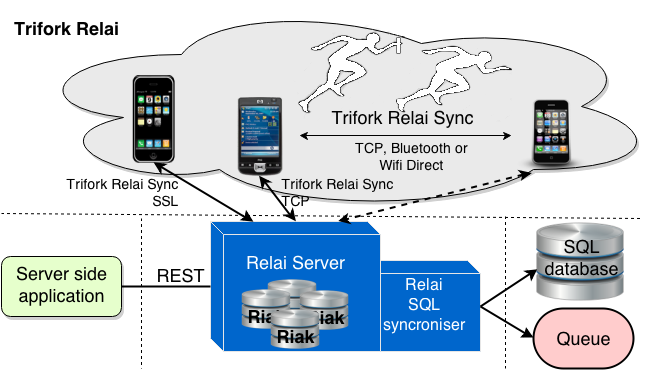
\includegraphics[width=1.05\textwidth]{figures/TriforkRelai.png}
	
	\caption{Overview of current Festival implementation which uses Trifork's Relai.}
	\label{fig:relai_layout}
\end{figure}

Massive events like conferences, sport events, and music festivals encounters may saturate the mobile bandwidth which would result in loss of cellular radio connectivity. Based on Trifork Relai local data are updated via not only cellular radio connectivity but also Blue-tooth and WiFi Direct with other devices in a peer-to-peer fashion. So although you may not be able to connect to a \gls{dc} you can still post your votes to peer devices just as you can get more up to date data from these.

Having a normal counter where you add one or more at the time will obviously not work in this scenario as we don't have a central database, we have no means to check how many times you are voting, nor do we have any means to see how large a percentage of possible votes have been given. This raises a new dilemma where the probabilistic counter comes in handy.

Each device will hold a bit array for voting bad and for voting good for each concert, i.e. when a vote is cast as ``bad'' a random number is generated on the device and the corresponding bit in the ``bad'' array is set. The same goes for the ``good'' votes, but note that each possible candidate (bad or good in this case) must have their own bit array. Now this array can be spread to peer devices where it is added to other device\textquoteright s bit arrays as a simple AND operation. At any device you can now see the total number of votes for bad and good by calculating the number of votes that are most likely with number of set bits compared to the number of still unset bits. This value will not change if an array is added several times, in other words it is idempotent. 

One consistency issue that is left unresolved is that you cannot see that few or many votes are missing. Obviously the precision of the count must be obtained by sizing the array towards the total number of votes cast. Another possible inconsistency is that segregated groups of devices can show uncorrelated results. This can happen in a number of situations which are unlikely but possible, i.e. lets say no cellular radio network is available and one group are now only networking using WiFi Direct and another group are only networking using Blue-tooth and no device is bridging the two means of networking. Then each group will have their own voting polls.

We have a number of unintended side effects. For a music festival this is acceptable, while for an App for parliament this would not be acceptable. In the implementation each device can only vote for each concert once and you cannot alter your vote after it has been given. If you have more devices you also have more votes. If you uninstall and reinstall the App you will be able to vote again for the same concert.

\subsubsection{Mark-Counter}
A Mark-Counter is composed of an array of $n$ bits. A Mark-Counter $B$ is composed of $n$ bits each represented by $B_{i} \in \{0, 1\} \forall i \in \{1,\dots, n\}$. $A^{n}$ represents the group of all the arrays of bits of size $n$ ($|B| = n$), where $n$ is also the number of bits in a Mark-Counter.

Bitwise OR operator is represented as | in this document.

{\bf Operations}:
\begin{itemize}
	\item \underline{Set} a bit in a Mark-Counter: a bit may change individually from 0 to 1 but may not be reset back to zero by this operator.
	
	\item \underline{Merge} Mark-Counters (bitwise OR operator, |): given two Mark-Counters $B, C \in A^{n}$, their merger is defined as $D = \{D_{i} = B_{i} | C_{i}, i \in \{1,\dots, n\}\}$.
	
	If both arrays have different sizes, i.e. $|B|$ and $|C|$, then $D = \{D_{i} = B_{i} | C_{i}, i \in \{1,\dots, \max{\{|B|, |C|\}}\}$ $\text{ with } B_{j} = 0 ~ \forall ~ j > |B|, C_{k} = 0 ~ \forall ~ k > |C|\}$ and the size of $D$ would be $|D| = \max{\{|B|, |C|\}}$.
	
	\item \underline{Count}: given a Mark-Counter $B$ the count corresponds to the number of bits that have been set to 1, $\sum^{|B|}_{i = 1} B_{i}$. Similarly, once it is know the number of 1s it is also known the number of zeros for a given array size.
\end{itemize}


{\bf A Mark-Counter is a \gls{crdt}}: A Mark-Counter is a simple data structure which complies with the requirements to be a \gls{crdt}, as shown below.
\begin{itemize}
	\item {\bf Commutative}. Given two Mark-Counts $B$ and $C$ with $n$ bits each where a bit index is presented by $i$ and its value in the Mark-Counter by $B_{i}$ and $C_{i}$ respectively the the merging of the corresponding bit at position $i$ provide the same result irrespective of the order the bit in each Mark-Counter is executed, as shown by, Equation \ref{eq:bit-counter_conmmutative}.
		\begin{equation}
			B_{i} | C_{i} = C_{i} | B_{i}
			\label{eq:bit-counter_conmmutative}
		\end{equation}
		
		The prove is shown on the Table \ref{tab:bit-counter_conmmutative} where the two first columns contain the input Mark-Counters and the last two columns the different order they may be computed which provide the same results.
		\begin{table}[!ht]
			\centering
			\begin{tabular}{|c|c||c|c|}
				\hline
				\multicolumn{2}{|c||}{Values} & \multicolumn{2}{|c|}{Results} \\
				\hline
				$B_{i}$ & $C_{i}$ & $B_{i}|C_{i}$ & $C_{i}|B_{i}$ \\
				\hline
				\hline
				0         & 0          & 0                  & 0             \\
				\hline
				1         & 0          & 1                  & 1             \\
				\hline
				0         & 1          & 1                  & 1             \\
				\hline
				1         & 1          & 1                  & 1             \\
				\hline
			\end{tabular}
			
			\caption{Mark-Counter commutative prove, $i \in \{1,\dots, n\}$.}
			\label{tab:bit-counter_conmmutative}
		\end{table}

	\item {\bf Associative}, Equation \ref{eq:bit-counter_associative}.
		\begin{equation}
			(B_{i} | C_{i}) | D_{i} = B_{i} | (C_{i} | D_{i})
			\label{eq:bit-counter_associative}
		\end{equation}
		
		The prove is shown on the Table \ref{tab:bit-counter_associative}.
		\begin{table}[!ht]
			\centering
			\begin{tabular}{|c|c|c||c|c||c|c|}
				\hline
				\multicolumn{3}{|c||}{Values} & \multicolumn{2}{|c||}{Intermediate} & \multicolumn{2}{|c|}{Results} \\
				\hline
				$B_{i}$ & $C_{i}$ & $D_{i}$ & $B_{i}|  C_{i}$ & $C_{i} | D_{i}$ & ($B_{i} | C_{i}) | D_{i}$ & $B_{i} | (C_{i}) | D_{i})$ \\
				\hline
				\hline
				0         & 0          & 0          & 0                    & 0                    & 0                                 & 0             \\
				\hline
				1         & 0          & 0          & 1                    & 0                    & 1                                 & 1             \\
				\hline
				0         & 1          & 0          & 1                    & 1                    & 1                                 & 1             \\
				\hline
				1         & 1          & 0          & 1                    & 1                    & 1                                 & 1             \\
				\hline
				0         & 0          & 1          & 0                    & 1                    & 1                                 & 1             \\
				\hline
				1         & 0          & 1          & 1                    & 1                    & 1                                 & 1             \\
				\hline
				0         & 1          & 1          & 1                    & 1                    & 1                                 & 1             \\
				\hline
				1         & 1          & 1          & 1                    & 1                    & 1                                 & 1             \\
				\hline
			\end{tabular}
			
			\caption{Mark-Counter associative prove, $i \in \{1,\dots, n\}$.}
			\label{tab:bit-counter_associative}
		\end{table}

	\item {\bf Idempotent}, Equation \ref{eq:bit-counter_idempotent}.
		\begin{equation}
			B_{i} | B_{i} = B_{i}
			\label{eq:bit-counter_idempotent}
		\end{equation}
		
		The prove is shown on the Table \ref{tab:bit-counter_idempotent}.
		\begin{table}[!ht]
			\centering
			\begin{tabular}{|c||c|c|c|}
				\hline
				Value   & Result             \\
				\hline
				$B_{i}$ & $B_{i} | B_{i} $ \\
				\hline
				\hline
				0         & 0                     \\
				\hline
				1         & 1                     \\
				\hline
			\end{tabular}
			
			\caption{Mark-Counter idempotent prove, $i \in \{1,\dots, n\}$.}
			\label{tab:bit-counter_idempotent}
		\end{table}
\end{itemize}


\subsubsection{Festival use case with Mark-Counters} 
Consider a "Festival" which it is composed of many acts/events. We start by considering the case of a "Festival" composed only of one act that later will be extended to many. To simplify, without losing generality, it is considered the case of an event in a theatre and the constants and variables used are presented in Table \ref{tab:festival_constants_variables}.
\begin{table*}[!ht]
	\begin{tabular}{|p{2.4cm}|p{11.2cm}|r| }
		\hline
		\multicolumn{1}{|c|}{Name} & \multicolumn{1}{c|}{Description} & \multicolumn{1}{c|}{Type} \\
		\hline
		\hline
%			$DC$ & It is a set of \glspl{dc} through which an event must be distributed and $d$ identifies one of the \gls{dc}, $d \in \{1,\dots, |DC|\}$. & $\mathbb{Z}_{+}$ \\
%		\hline
			$People$ & It is the set of people attending the "Festival" and $p$ represent one of those people ($p \in People$), with $|People|$ representing the number of people attending and the size of the array of bits. & $p \in \mathbb{Z}_{+}$ \\
		\hline
			$n_{d}$ & It refers to the highest attendee's index to the "Festival" that the device $d$ has information about,  $d \in \{1,\dots, |People|\}$. Also $1 \le n_{d} \le |People| ~ \forall ~ d \in \{1,\dots, |People|\}$. & $\mathbb{Z}_{+}$ \\
		\hline
			$G_{d}$ & It is the array of good votes known by the device $d$ from device $d$ and other devices. $G_{d}$ is an array of bit of size of at least $n_{d}$, with each bit represent a device. $G_{d}$ is a Mark-Counter where a bit is set to 1 if the corresponding attendee, represented by that bit, is set to 1 to state the vote of the attendee as good. & $\mathbb{Z}_{+}$ \\
		\hline 
			$G_{da}$ & It is the value in the array of good votes available at devise $d$ for attendee $a$, presented in Expression \ref{ep:good_values}. Also it can be said to be the bit $a$ in the array of bits $G_{d}$, $a \in \{1,\dots, |People|\}$.
				\begin{equation} \label{ep:good_values}
					0 \le G_{ka} \le 1 ~ \forall k,a \in \{1,\dots, |People|\}
				\end{equation} & 
			$\mathbb{Z}_{+}$ \\
		\hline
			$B_{d}$ & It is the array of bad votes known by device $d$ from device $d$ and other devices. $B_{d}$ is an array of bit of size of at least $n_{d}$, with each bit represent a device. $B_{d}$ is a Mark-Counter where a bit is set to 1 if the corresponding attendee, represented by that bit, is set to 1 to state the vote of the attendee as bad. & $\mathbb{Z}_{+}$ \\
		 \hline
		 	$B_{da}$ & It is the value in the array of bad votes seen by device $d$ for attendee $a$, $B_{da}$, presented in Expression \ref{ep:bad_values}. Also it can be said to be the bit $a$ in the array of bits $B_{d}$, $a \in \{1,\dots, |People|\}$.
				\begin{equation} \label{ep:bad_values}
					0 \le B_{da} \le 1 ~ \forall d, a \in \{1,\dots, |People|\}
				\end{equation} & 
			$\mathbb{Z}_{+}$ \\
		\hline
			$numGood_{d}$ & It is the number of good votes received by the attendee $d$ device, as shown by Equation \ref{eq:local_total_good_votes}. & $\mathbb{Z}_{+}$ \\
		\hline
			$numGood$ & It represents the total number of attendees that voted good, as shown in Equations  \ref{eq:attendee_voted_good} and \ref{eq:total_good_votes}. It is considered that if $n_{d} < |People|$ then $G_{da} = B_{da} = 0 ~ \forall ~ a > n_{d}$. & $\mathbb{Z}_{+}$ \\
		\hline
			$numBad_{d}$ & It is the number of bad votes received by the attendee $d$ device, as shown by Equation \ref{eq:local_total_bad_votes}. & $\mathbb{Z}_{+}$ \\
		\hline
			$numBad$ & It represents the total number of attendees that voted bad, as shown in Equations \ref{attendee_voted_bad} and \ref{eq:total_bad_votes}. & $\mathbb{Z}_{+}$ \\
		\hline
			$numAttendees_{d}$ & It represents the total number of attendees that voted as seen by device/attendee $d$, as shown in Equation \ref{eq:num_votes}. & $\mathbb{Z}_{+}$ \\
		\hline
			$numAttendees$ & It represents the total number of attendees that voted, as shown in Equation \ref{eq:total_num_votes}. & $\mathbb{Z}_{+}$ \\
		\hline
	\end{tabular}
			
	\caption{Festival Constants and Variables.}
	\label{tab:festival_constants_variables}
\end{table*}
\begin{equation} \label{eq:attendee_voted_good}
	\delta^{good}_{d} = \left\{\begin{array}{ll}
		1 & if \sum_{a \in People} G_{da} > 0\\
		0 & otherwise
	\end{array}
	\right.
\end{equation}
\begin{equation} \label{eq:total_good_votes}
	numGood  = \sum_{d \in People} \delta^{good}_{d}
\end{equation}
\begin{equation} \label{eq:local_total_good_votes}
	numGood_{d}  = \sum^{n_{d}}_{a=1} G_{da} ~ \forall ~ d \in \{1,\dots, |People|\}
\end{equation}
\begin{equation} \label{attendee_voted_bad}
	\delta^{bad}_{d} = \left\{\begin{array}{ll}
		1 & if \sum_{d \in People} B_{da} > 0\\
		0 & otherwise
	\end{array}
	\right.
\end{equation}
\begin{equation} \label{eq:total_bad_votes}
	numBad  = \sum_{d \in People} \delta^{bad}_{d}
\end{equation}
\begin{equation} \label{eq:local_total_bad_votes}
	numBad_{d}  = \sum^{n_{d}}_{a=1} B_{da} ~ \forall ~ d \in \{1,\dots, |People|\}
\end{equation}
\begin{equation} \label{eq:num_votes}
	numAttendees_{d}  = \sum^{n_{d}}_{a=1} (G_{da} + B_{da}) ~ \forall ~ d \in \{1,\dots, |People|\}
\end{equation}
\begin{equation} \label{eq:total_num_votes}
	numAttendees  = numGood + numBad
\end{equation}

An attendee may only vote once as expressed in Inequality \ref{ep:vote_not_equal}, but he/she may not vote at all.
\begin{equation} \label{ep:vote_not_equal}
	G_{da} + B_{da} < 2 ~ \forall ~ d \in \{1,\dots, |People|\}, a \in \{1,\dots, n_{k}\}
\end{equation}

A measure of the coherence for the copies between an attendee $a$ and another attendee $j$ can be obtained by calculating the number of bits where both versions of voting differ as expressed in Equation \ref{eq:discrepancy_votes}. All the devices are in sync if $\bigtriangleup numAttendees_{dj} = 0 ~ \forall ~ d, j \in \{1,\dots, |People|\}$.
\begin{equation} \label{eq:discrepancy_votes}
	\bigtriangleup numAttendees_{dj} = \sum_{i \in People} ((G_{di} + G_{ji}) \% 2 + (B_{dj} + B_{ji}) \% 2) \forall ~ d, j \in \{1,\dots, |People|\}
\end{equation}

This can be extended to multiple events/acts by introducing a new index that represent each of these events/acts.

The problem with the real Festival use case is that not all devices may know about all the attendees and even if they did then the size of the bit arrays may be too big to be efficient their use, so Trifork come with the idea of using Statistical Mark-Counter. which are presented in Section \ref{sec:stat_mark_counter}. In Trifork's Festival the counters are reduced in size by using statistics, and each bit is randomly assigned to a customer.

\subsubsection{Statistical Mark-Counter} \label{sec:stat_mark_counter}
To reduce the amount of data transferred between devices and for cases where not all devises may know the total number of attendees it could be used a probabilistic approach. The current Trifork's Festival implementation already uses an statistical Mark-Counter, where the index of an attendee is calculated randomly for a pre-defined size of the poll, $n_{d} = n \le |People| ~ \forall ~ d \in \{1,\dots, n\}$. This means that different attendees may be assigned the same position in the poll, so potentially their votes would equate to a single vote, if they vote equally. So given this the Inequality \ref{ep:vote_less_equal} would not be complied with so it would needs to be removed from the representation to \ref{attendee_voted_bad}.
\begin{equation} \label{ep:vote_less_equal}
	G_{da} + B_{da} \le 2 ~ \forall ~ d, a \in \{1,\dots, n\}
\end{equation}

The size of the array of bits depends of the quality expected from the results extrapolated, whereas larger sizes generally lead to increased precision, e.g. a size equal to the number of attendees will provide the maximum precision. In practice, the size used in a study is determined based on the cost of data collection, storage, transmission, processing, and the need to have sufficient statistical power. Sizes may be chosen in several different ways such as target for the power and target variance of a statistical test.


\ifnum\firstUserCase=1
	\newpage
\fi
\section{Business to Business (B2B)}
This application was built from the ground up for a large clothes manufacturer, who sells boxes of clothes to thousands of stores in 30+ markets. It replaces a manual process, where travelling salesmen visited the stores and presented physical clothing from their sample collections.

The \gls{b2b} order application enables the clients, e.g. shop employees, to see a catalogue of upcoming clothes on a tablet device, and place orders on boxes for future delivery. This functionality is made available for the same shops to shop staff as well as for shop managers, managers of chains of shops or managers of entire markets. Orders are modelled as a \gls{gset} \cite{shapiro11comprehensive}, which is updated by adding event objects.

The tablets can operate off-line and only need to be online for getting i.e. new catalogue replicated down and for posting orders towards the server. It is expected that stores cannot be spread over many \glspl{dc}. More \glspl{dc} can be used and in this case each \gls{dc} must be aware of in which \gls{dc} each shop's data is located.

The tablets can remain off-line for any length of time. This effectively means that there will be issues with double orders, out of stock, not current catalogue, and other conflicts. The automated system is not intended for handling these conflicts while it will attempt to detect conflicts and potential conflicts. These will then be brought to the attention of manufacturer's customer support.

Cancellation and adjustment of orders are not offered via the tablet solution. These will have to be dealt with by the manufacturers customer support.




\ifnum\firstUserCase=1
%	\cleardoublepage
	\newpage
\fi
\section{Conclusion}
We have seen databases residing in one \gls{dc}, in replicated \glspl{dc}, on mobile phones, and distributed across all with potential eventual consistency. But we have also seen how data is present at the point of entry and possible believed by the user to be persistent in a ``central'' although maybe never delivered. These scenarios represents the \glspl{crdt} at 
\begin{itemize}
	\item Server side
	\item Points-of-presence
	\item Edge of network
\end{itemize}
The attributes of the data in process
\begin{itemize}
	\item Object composition and transaction
	\item Divergence and Quality of data
	\item Security
\end{itemize}
Some of the requirements we have looked at will be supported early and can be verified in the basic programming model. Others are more comprehensive and cannot be expected to be successfully verified until later. Eventually some requirements will not be satisfied as they are not feasible in an automatic context.
\begin{itemize}
	\item Basic programming model
	\item Extended programming model
	\item Final programming model
\end{itemize}
All of the examples use as input to the requirement gathering are from the real world and they amongst others represent a world wide hundred billion Euro electronic entertainment industry and the Health Care Sector taking a two digit percentile of Western State Budgets. The present IT Industry have very little support for this kind of applications and as we have seen the problems addressed in the use cases are not supported in classic database implementations.


%ACKNOWLEDGMENTS are optional
%\section{Acknowledgements}
%This has been created as part of the European research project \href{https://syncfree.lip6.fr}{SyncFree}.

\ifnum\firstUserCase=1
%	\cleardoublepage
\newpage
\fi


%
% The following two commands are all you need in the initial runs of your .tex file to produce the bibliography for the citations in your paper.
\bibliographystyle{abbrv}
\bibliography{../syncFree}  % sigproc.bib is the name of the Bibliography in this case
% You must have a proper ".bib" file and remember to run:
% latex bibtex latex latex to resolve all references
%
% ACM needs 'a single self-contained file'!
%

%APPENDICES are optional
%\balancecolumns
%\appendix
%Appendix A

\balancecolumns
% That's all
\ifnum\withAppendix=1

\onecolumn
\appendix

\section{TLA+ representation of Use Cases}
\vspace{.5em}
\begin{enumerate}
	\item Advertisement Counter
	\item Leader Board
	\item Virtual Wallet
	\item Shared Medicine Record (FMK) 
	\item Festival
	\item Business to Business (B2B)
\end{enumerate}


\subsection{Advertisement Counter (AdCounter)}\label{use_case_ad_counter}

\verbinput{TLA/adCounter_v2.tla}


\subsection{Leader Board}\label{use_case_leader_board}

\verbinput{TLA/leaderBoard_v2.tla}


\subsection{Virtual Wallet}\label{use_case_virtual_wallet}


%\begin{document}
\tlatex
\@x{}\moduleLeftDash\@xx{ {\MODULE} walletv4}\moduleRightDash\@xx{}%
\@x{ {\EXTENDS} Naturals ,\, Sequences ,\, TLC}%
\@x{ {\VARIABLES} wallets}%
\@x{ {\CONSTANTS} Replicas ,\, V1Cost ,\, InitBal ,\, Natlim ,\, Qtylim}%
\@pvspace{8.0pt}%
\@x{ {\ASSUME} \.{\land} V1Cost \.{\in} Nat}%
\@x{\@s{38.24} \.{\land} InitBal \.{\in} Nat}%
\@x{\@s{38.24} \.{\land} Natlim\@s{4.46} \.{\in} Nat}%
\@x{\@s{38.24} \.{\land} Qtylim\@s{4.48} \.{\in} Nat}%
\@x{\@s{38.24} \.{\land} V1Cost \.{>} 0}%
\@x{\@s{38.24} \.{\land} Natlim\@s{4.46} \.{>} 0}%
\@x{\@s{38.24} \.{\land} Qtylim\@s{4.48} \.{>} 0}%
\@x{}\midbar\@xx{}%
\@pvspace{8.0pt}%
 \@x{ PNCounter ( dom ) \.{\defeq} [ p\@s{0.64} \.{:} [ dom \.{\rightarrow}
 Nat ] ,\,}%
\@x{\@s{99.29} n \.{:} [ dom \.{\rightarrow} Nat ] ]}%
\@pvspace{8.0pt}%
 \@x{ InitPNCounter ( dom ) \.{\defeq} [ p \.{\mapsto} [ d \.{\in} dom
 \.{\mapsto} 0 ] ,\, n \.{\mapsto} [ d \.{\in} dom \.{\mapsto} 0 ] ]}%
\@pvspace{16.0pt}%
\@x{ SumAll ( map ) \.{\defeq}}%
 \@x{\@s{16.4} \.{\LET} Sum [ r \.{\in} {\SUBSET} {\DOMAIN} map ] \.{\defeq}
 {\IF} r \.{=} \{ \} \.{\THEN} 0 \.{\ELSE} \.{\LET} y \.{\defeq} {\CHOOSE} x
 \.{\in} r \.{:} {\TRUE} \.{\IN} map [ y ] \.{+} Sum [ r \.{\,\backslash\,}
 \{ y \} ]}%
\@x{\@s{16.4} \.{\IN} Sum [ {\DOMAIN} map ]}%
\@pvspace{8.0pt}%
 \@x{ EvalPNCounter ( pnc ) \.{\defeq} SumAll ( pnc . p ) \.{-} SumAll ( pnc .
 n )}%
\@pvspace{8.0pt}%
 \@x{ Max ( n1 ,\, n2 ) \.{\defeq} {\IF} n1 \.{\geq} n2 \.{\THEN} n1 \.{\ELSE}
 n2}%
\@pvspace{8.0pt}%
 \@x{ MergePNCounters ( pnc1 ,\, pnc2 ) \.{\defeq} [ p \.{\mapsto} [ d \.{\in}
 {\DOMAIN} pnc1 . p \.{\mapsto} Max ( pnc1 . p [ d ] ,\, pnc2 . p [ d ] ) ]
 ,\, n \.{\mapsto} [ d \.{\in} {\DOMAIN} pnc1 . n \.{\mapsto} Max ( pnc1 . n
 [ d ] ,\, pnc2 . n [ d ] ) ] ]}%
\@pvspace{8.0pt}%
\@x{}\midbar\@xx{}%
\@pvspace{8.0pt}%
\@x{ Wallet \.{\defeq} [ balance \.{:} PNCounter ( Replicas ) ,\,}%
\@x{\@s{51.25} v1cnt \.{:} PNCounter ( Replicas ) ,\,}%
\@x{\@s{51.25} vecclc \.{:} [ Replicas \.{\rightarrow} Nat ] ]}%
\@pvspace{16.0pt}%
 \@x{ TypeInv \.{\defeq} \.{\land} wallets \.{\in} [ Replicas \.{\rightarrow}
 Seq ( Wallet ) ]}%
\@pvspace{16.0pt}%
\@x{ Init \.{\defeq}}%
\@y{%
 \ensuremath{\.{\land} Print} (``a'', \ensuremath{{\TRUE}})
}%
\@xx{}%
 \@x{\@s{35.70} \.{\land} wallets \.{=} [ r \.{\in} Replicas \.{\mapsto}
 {\langle} [ balance \.{\mapsto} InitPNCounter ( Replicas ) ,\,}%
\@x{\@s{167.43} v1cnt\@s{4.1} \.{\mapsto} InitPNCounter ( Replicas ) ,\,}%
 \@x{\@s{167.43} vecclc\@s{4.17} \.{\mapsto} [ r2 \.{\in} Replicas \.{\mapsto}
 0 ] ] {\rangle} ]}%
\@pvspace{16.0pt}%
\@x{ App ( elt ,\, s ) \.{\defeq} {\langle} elt {\rangle} \.{\circ} s}%
\@pvspace{8.0pt}%
\@x{ BuyV1 ( rep ,\, qty ) \.{\defeq}}%
\@x{\@s{16.4} \.{\LET} wr \.{\defeq} Head ( wallets [ rep ] )}%
 \@x{\@s{36.79} new\_bal\_n \.{\defeq} [ wr . balance . n {\EXCEPT} {\bang} [
 rep ] \.{=} wr . balance . n [ rep ] \.{+} qty \.{*} V1Cost ]}%
 \@x{\@s{36.79} new\_v1\_cnt\_p \.{\defeq} [ wr . v1cnt . p {\EXCEPT} {\bang}
 [ rep ] \.{=} wr . v1cnt . p [ rep ] \.{+} qty ]}%
 \@x{\@s{36.79} new\_vc\@s{2.17} \.{\defeq} [ wr . vecclc {\EXCEPT} {\bang} [
 rep ] \.{=} wr . vecclc [ rep ] \.{+} 1 ]}%
 \@x{\@s{36.79} wr\_new \.{\defeq} [ balance \.{\mapsto} [ p \.{\mapsto} wr .
 balance . p ,\, n \.{\mapsto} new\_bal\_n ] ,\,}%
 \@x{\@s{92.84} v1cnt \.{\mapsto} [ p \.{\mapsto} new\_v1\_cnt\_p ,\, n
 \.{\mapsto} wr . v1cnt . n ] ,\,}%
\@x{\@s{92.84} vecclc \.{\mapsto} new\_vc ]}%
 \@x{\@s{16.4} \.{\IN} \.{\land} wr . balance . n [ rep ] \.{+} qty \.{*}
 V1Cost \.{\leq} Natlim}%
\@x{\@s{36.79} \.{\land} wr . v1cnt . p [ rep ] \.{+} qty \.{\leq} Natlim}%
\@x{\@s{36.79} \.{\land} wr . vecclc [ rep ] \.{+} 1 \.{\leq} Natlim}%
 \@x{\@s{36.79} \.{\land} EvalPNCounter ( wr . balance ) \.{+} InitBal
 \.{\geq} qty \.{*} V1Cost}%
 \@x{\@s{36.79} \.{\land} wallets \.{'} \.{=} [ wallets {\EXCEPT} {\bang} [
 rep ]\@s{22.45} \.{=} App ( wr\_new ,\, wallets [ rep ] ) ]}%
\@x{\@s{36.79} \.{\land} Print (\@w{Buy} ,\, {\TRUE} )}%
\@x{\@s{24.59}}%
\@y{\@s{0}%
 \ensuremath{\.{\land} Print(wallets\.{'},\, {\TRUE})
}}%
\@xx{}%
\@pvspace{8.0pt}%
 \@x{ GetElt ( seq ,\, ind ) \.{\defeq} Head ( SubSeq ( seq ,\, ind ,\, ind )
 )}%
\@pvspace{8.0pt}%
\@x{ Merge ( rep1 ,\, rep2 ,\, ind ) \.{\defeq}}%
\@x{\@s{16.4} \.{\LET} wr1 \.{\defeq} Head ( wallets [ rep1 ] )}%
\@x{\@s{36.79} wr2 \.{\defeq} GetElt ( wallets [ rep2 ] ,\, ind )}%
 \@x{\@s{36.79} new\_vc \.{\defeq} [ r \.{\in} Replicas \.{\mapsto} Max ( wr1
 . vecclc [ r ] ,\, wr2 . vecclc [ r ] ) ]}%
 \@x{\@s{36.79} wr1\_new \.{\defeq} [ balance \.{\mapsto} MergePNCounters (
 wr1 . balance ,\, wr2 . balance ) ,\,}%
 \@x{\@s{97.84} v1cnt \.{\mapsto} MergePNCounters ( wr1 . v1cnt ,\, wr2 .
 v1cnt ) ,\,}%
\@x{\@s{97.84} vecclc \.{\mapsto} new\_vc ]}%
 \@x{\@s{16.4} \.{\IN} \.{\land} \E\, r \.{\in} Replicas \.{:} wr1 . vecclc [
 r ] \.{<} wr2 . vecclc [ r ]}%
 \@x{\@s{36.79} \.{\land} wallets \.{'} \.{=} [ wallets {\EXCEPT} {\bang} [
 rep1 ] \.{=} App ( wr1\_new ,\, wallets [ rep1 ] ) ]}%
\@x{\@s{36.79} \.{\land} Print (\@w{Merge} ,\, {\TRUE} )}%
\@x{\@s{36.79}}%
\@y{%
 \ensuremath{\.{\land} Print(wallets\.{'},\, {\TRUE})
}}%
\@xx{}%
\@pvspace{8.0pt}%
\@x{ MergeLastStates ( rep1 ,\, rep2 ) \.{\defeq}}%
\@x{\@s{16.4} \.{\LET} wr1 \.{\defeq} Head ( wallets [ rep1 ] )}%
\@x{\@s{36.79} wr2 \.{\defeq} Head ( wallets [ rep2 ] )}%
 \@x{\@s{36.79} new\_vc \.{\defeq} [ r \.{\in} Replicas \.{\mapsto} Max ( wr1
 . vecclc [ r ] ,\, wr2 . vecclc [ r ] ) ]}%
 \@x{\@s{36.79} wr1\_new \.{\defeq} [ balance \.{\mapsto} MergePNCounters (
 wr1 . balance ,\, wr2 . balance ) ,\,}%
 \@x{\@s{97.84} v1cnt \.{\mapsto} MergePNCounters ( wr1 . v1cnt ,\, wr2 .
 v1cnt ) ,\,}%
\@x{\@s{97.84} vecclc \.{\mapsto} new\_vc ]}%
 \@x{\@s{16.4} \.{\IN} \.{\land} \E\, r \.{\in} Replicas \.{:} wr1 . vecclc [
 r ] \.{<} wr2 . vecclc [ r ]}%
 \@x{\@s{36.79} \.{\land} wallets \.{'} \.{=} [ wallets {\EXCEPT} {\bang} [
 rep1 ] \.{=} App ( wr1\_new ,\, wallets [ rep1 ] ) ]}%
\@x{\@s{36.79} \.{\land} Print (\@w{MergeLastStates} ,\, {\TRUE} )}%
\@x{\@s{36.79}}%
\@y{%
 \ensuremath{\.{\land} Print(wallets\.{'},\, {\TRUE})
}}%
\@xx{}%
\@pvspace{16.0pt}%
\@x{}%
\@y{\@s{0}%
 Amount of Money spent should be equal to the number of vouchers bought times
 the unit cost of the voucher in each replica
}%
\@xx{}%
 \@x{ ConservationOfMoney \.{\defeq} \A\, r \.{\in} Replicas \.{:}
 EvalPNCounter ( Head ( wallets [ r ] ) . balance )\@s{4.1} \.{+}
 EvalPNCounter ( Head ( wallets [ r ] ) . v1cnt ) \.{*} V1Cost \.{=} 0}%
\@pvspace{8.0pt}%
\@x{}%
\@y{\@s{0}%
 Balance in the wallet is always positive \cdash{3} DOES NOT HOLD
}%
\@xx{}%
 \@x{ PosBalance \.{\defeq} \A\, rep \.{\in} Replicas \.{:} InitBal \.{+}
 EvalPNCounter ( Head ( wallets [ rep ] ) . balance ) \.{\geq} 0}%
\@pvspace{8.0pt}%
\@x{}%
\@y{\@s{0}%
 Fields of \ensuremath{P} and \ensuremath{N} fields of \ensuremath{PN}
 counters and vector clocks are monotonically nondecreasing in time
}%
\@xx{}%
 \@x{ Monotonicity \.{\defeq} \.{\land} \A\, r \.{\in} Replicas ,\, r2 \.{\in}
 Replicas ,\, i \.{\in} Nat \.{:} ( i \.{>} 0 \.{\land} i \.{<} Len ( wallets
 [ r ] ) ) \.{\implies} ( GetElt ( wallets [ r ] ,\, i ) . vecclc [ r2 ]
 \.{\geq} GetElt ( wallets [ r ] ,\, i \.{+} 1 ) . vecclc [ r2 ]}%
 \@x{\@s{397.89} \.{\land} GetElt ( wallets [ r ] ,\, i ) . balance . p [ r2
 ]\@s{0.64} \.{\geq} GetElt ( wallets [ r ] ,\, i \.{+} 1 ) . balance . p [
 r2 ]}%
 \@x{\@s{397.89} \.{\land} GetElt ( wallets [ r ] ,\, i ) . balance . n [ r2 ]
 \.{\geq} GetElt ( wallets [ r ] ,\, i \.{+} 1 ) . balance . n [ r2 ]}%
 \@x{\@s{397.89} \.{\land} GetElt ( wallets [ r ] ,\, i ) . v1cnt . p [ r2
 ]\@s{0.64} \.{\geq} GetElt ( wallets [ r ] ,\, i \.{+} 1 ) . v1cnt . p [ r2
 ]}%
 \@x{\@s{397.89} \.{\land} GetElt ( wallets [ r ] ,\, i ) . v1cnt . n [ r2 ]
 \.{\geq} GetElt ( wallets [ r ] ,\, i \.{+} 1 ) . v1cnt . n [ r2 ] )}%
\@pvspace{8.0pt}%
 \@x{ FinalState ( vc ) \.{\defeq} \A\, rep \.{\in} Replicas \.{:} vc [ rep ]
 \.{=} Natlim}%
 \@x{ EqualStates ( st1 ,\, st2 ) \.{\defeq} \A\, rep \.{\in} Replicas \.{:}
 st1 . balance . p [ rep ] \.{=} st2 . balance . p [ rep ] \.{\land} st1 .
 balance . n [ rep ] \.{=} st2 . balance . n [ rep ] \.{\land} st1 . v1cnt .
 p [ rep ] \.{=} st2 . v1cnt . p [ rep ] \.{\land} st1 . v1cnt . n [ rep ]
 \.{=} st2 . v1cnt . n [ rep ]}%
\@x{}%
\@y{\@s{0}%
 Eventually all states converge to the same state
}%
\@xx{}%
 \@x{ Convergence \.{\defeq} \A\, r1 \.{\in} Replicas ,\, r2 \.{\in} Replicas
 \.{:} FinalState ( Head ( wallets [ r1 ] ) . vecclc ) \.{\land} FinalState (
 Head ( wallets [ r2 ] ) . vecclc ) \.{\implies} EqualStates ( Head ( wallets
 [ r1 ] ) ,\, Head ( wallets [ r2 ] ) )}%
\@pvspace{8.0pt}%
 \@x{ Next \.{\defeq} \E\, r1 \.{\in} Replicas ,\, r2 \.{\in} Replicas ,\, qty
 \.{\in} 1 \.{\dotdot} Qtylim}%
\@y{%
 , \ensuremath{i \.{\in} Nat
}}%
\@xx{ \.{:}}%
\@y{%
 \ensuremath{i \.{\leq} Len(wallets[r2]) \.{\land} i \.{>}0 \.{\land}
}}%
\@xx{ ( BuyV1 ( r1 ,\, qty ) \.{\lor}}%
\@y{%
 \ensuremath{Merge(r1,\,r2,\,i)
}}%
\@xx{ MergeLastStates ( r1 ,\, r2 ) )}%
\@pvspace{8.0pt}%
 \@x{ Spec\@s{1.46} \.{\defeq} Init \.{\land} {\Box} [ Next ]_{ {\langle}
 wallets {\rangle}}}%
\@pvspace{8.0pt}%
\@x{ {\THEOREM} Spec \.{\implies} TypeInv \.{\land} ConservationOfMoney}%
\@x{}\bottombar\@xx{}%
%\end{document}


\subsubsection{Wallet use case using Integers}
The balance and the counts of the vouchers in the wallets are integers instead of PN-Counters. When two copies of a wallet account are merged the maximum of the balances of the wallets is taken so the balance is generous for the player. When merging the total count of vouchers, the amount of vouchers is added in the two copies. As expected, when it is tested in TLC some money is lost, i.e. the total money spend is more than the money reduced from the balance. The TLA+ representation for this particular example is presented bellow.

\tlatex
\@x{}\moduleLeftDash\@xx{ {\MODULE} walletNat}\moduleRightDash\@xx{}%
\@x{ {\EXTENDS} Integers ,\, TLC ,\, Naturals}%
\@x{ {\VARIABLE} wallets}%
\@x{ {\CONSTANTS} Replicas ,\, V1Cost ,\, InitBal ,\, Natlim ,\, Qtylim}%
\@pvspace{8.0pt}%
\@x{}\midbar\@xx{}%
\@pvspace{8.0pt}%
\@x{ Wallet \.{\defeq} [ balance \.{:} Int ,\,}%
\@x{\@s{51.25} v1cnt \.{:} Int ,\,}%
\@x{\@s{51.25} vecclc \.{:} [ Replicas \.{\rightarrow} Nat ] ]}%
\@pvspace{8.0pt}%
 \@x{ TypeInv \.{\defeq} \.{\land} wallets \.{\in} [ Replicas \.{\rightarrow}
 Wallet ]}%
\@pvspace{8.0pt}%
 \@x{ Init \.{\defeq}\@s{4.1} \.{\land} wallets \.{=} [ r \.{\in} Replicas
 \.{\mapsto} [ balance \.{\mapsto} InitBal ,\,}%
\@x{\@s{170.42} v1cnt \.{\mapsto} 0 ,\,}%
\@x{\@s{170.42} vecclc \.{\mapsto} [ r2 \.{\in} Replicas \.{\mapsto} 0 ] ] ]}%
\@x{\@s{29.11} \.{\land} Print ( wallets ,\, {\TRUE} )}%
\@pvspace{8.0pt}%
\@x{ BuyV1 ( rep ,\, qty ) \.{\defeq}}%
\@x{\@s{16.4} \.{\LET} wr \.{\defeq} wallets [ rep ]}%
 \@x{\@s{36.79} new\_vc\@s{2.17} \.{\defeq} [ wr . vecclc {\EXCEPT} {\bang} [
 rep ] \.{=} wr . vecclc [ rep ] \.{+} 1 ]}%
 \@x{\@s{36.79} new\_wr \.{\defeq} [ balance \.{\mapsto} wr . balance \.{-}
 qty \.{*} V1Cost ,\,}%
\@x{\@s{92.84} v1cnt \.{\mapsto} wr . v1cnt \.{+} qty ,\,}%
\@x{\@s{92.84} vecclc \.{\mapsto} new\_vc ]}%
\@x{\@s{16.4} \.{\IN} \.{\land} wr . balance \.{\geq} qty \.{*} V1Cost}%
\@x{\@s{36.79} \.{\land} wr . v1cnt \.{+} qty \.{\leq} Natlim}%
\@x{\@s{36.79} \.{\land} wr . vecclc [ rep ] \.{+} 1 \.{\leq} Natlim}%
 \@x{\@s{36.79} \.{\land} wallets \.{'}\@s{18.09} \.{=} [ wallets {\EXCEPT}
 {\bang} [ rep ] \.{=} new\_wr ]}%
\@pvspace{8.0pt}%
 \@x{ Max ( n1 ,\, n2 ) \.{\defeq} {\IF} n1 \.{\geq} n2 \.{\THEN} n1 \.{\ELSE}
 n2}%
\@pvspace{8.0pt}%
\@x{ Merge ( r1 ,\, r2 ) \.{\defeq}}%
\@x{\@s{16.4} \.{\LET} wr1 \.{\defeq} wallets [ r1 ]}%
\@x{\@s{36.79} wr2 \.{\defeq} wallets [ r2 ]}%
 \@x{\@s{36.79} new\_vc\@s{2.95} \.{\defeq} [ r \.{\in} Replicas \.{\mapsto}
 Max ( wr1 . vecclc [ r ] ,\, wr2 . vecclc [ r ] ) ]}%
 \@x{\@s{36.79} new\_w1 \.{\defeq} [ balance \.{\mapsto} Max ( wr1 . balance
 ,\, wr2 . balance ) ,\,}%
\@x{\@s{93.62} v1cnt \.{\mapsto} Max ( wr1 . v1cnt ,\, wr2 . v1cnt ) ,\,}%
\@y{\@s{0}%
 alternative formulation: \ensuremath{wr1.v1cnt\.{+}wr2.v1cnt
}}%
\@xx{}%
\@x{\@s{93.62} vecclc \.{\mapsto} new\_vc ]}%
\@pvspace{8.0pt}%
 \@x{\@s{16.4} \.{\IN} \.{\land} \E\, r \.{\in} Replicas \.{:} wr1 . vecclc [
 r ] \.{<} wr2 . vecclc [ r ]}%
 \@x{\@s{36.79} \.{\land} wallets \.{'} \.{=} [ wallets {\EXCEPT} {\bang} [ r1
 ] \.{=} new\_w1 ]}%
\@pvspace{16.0pt}%
 \@x{ ConservationOfMoney \.{\defeq} \A\, r \.{\in} Replicas \.{:} ( InitBal
 \.{-} wallets [ r ] . balance ) \.{\geq} wallets [ r ] . v1cnt \.{*} V1Cost}%
\@pvspace{8.0pt}%
 \@x{ FinalState ( vc ) \.{\defeq} \A\, r \.{\in} Replicas \.{:} vc [ r ]
 \.{=} Natlim}%
 \@x{ EqualStates ( st1 ,\, st2 ) \.{\defeq} st1 . balance \.{=} st2 . balance
 \.{\land} st1 . v1cnt \.{=} st2 . v1cnt}%
 \@x{ Convergence \.{\defeq} \A\, r1 \.{\in} Replicas ,\, r2 \.{\in} Replicas
 \.{:}}%
 \@x{\@s{32.8} FinalState ( wallets [ r1 ] . vecclc ) \.{\land} FinalState (
 wallets [ r2 ] . vecclc ) \.{\implies}}%
\@x{\@s{65.6} EqualStates ( wallets [ r1 ] ,\, wallets [ r2 ] )}%
\@pvspace{8.0pt}%
 \@x{ Next \.{\defeq} \E\, r1 \.{\in} Replicas ,\, r2 \.{\in} Replicas ,\, qty
 \.{\in} 1 \.{\dotdot} Qtylim \.{:} ( BuyV1 ( r1 ,\, qty ) \.{\lor} Merge (
 r1 ,\, r2 ) )}%
\@pvspace{8.0pt}%
 \@x{ Spec\@s{1.46} \.{\defeq} Init \.{\land} {\Box} [ Next ]_{ {\langle}
 wallets {\rangle}}}%
\@pvspace{8.0pt}%
 \@x{ {\THEOREM} Spec \.{\implies} TypeInv \.{\land} ConservationOfMoney
 \.{\land} Convergence}%
\@x{}\bottombar\@xx{}%

\subsubsection{Wallet use case using No Atomic Operations}
In here it is presented the scenario in which buying some vouchers is not an atomic operation. For this model, it is defined two operators so that PN-Counters, which keep the balance and voucher counts, could be merged separately. As expected again, some money is lost and some properties are not satisfied. The TLA+ representation for this particular example is presented bellow.

\batchmode %% Suppresses most terminal output.
\documentclass{article}
\setlength{\textwidth}{360pt}
\setlength{\textheight}{541pt}
\usepackage{latexsym}
\usepackage{ifthen}
% \usepackage{color}
%%%%%%%%%%%%%%%%%%%%%%%%%%%%%%%%%%%%%%%%%%%%%%%%%%%%%%%%%%%%%%%%%%%%%%%%%%%%%
% SWITCHES                                                                  %
%%%%%%%%%%%%%%%%%%%%%%%%%%%%%%%%%%%%%%%%%%%%%%%%%%%%%%%%%%%%%%%%%%%%%%%%%%%%%
\newboolean{shading} 
\setboolean{shading}{false}
\makeatletter
 %% this is needed only when inserted into the file, not when
 %% used as a package file.
%%%%%%%%%%%%%%%%%%%%%%%%%%%%%%%%%%%%%%%%%%%%%%%%%%%%%%%%%%%%%%%%%%%%%%%%%%%%%
%                                                                           %
% DEFINITIONS OF SYMBOL-PRODUCING COMMANDS                                  %
%                                                                           %
%    TLA+      LaTeX                                                        %
%    symbol    command                                                      %
%    ------    -------                                                      %
%    =>        \implies                                                     %
%    <:        \ltcolon                                                     %
%    :>        \colongt                                                     %
%    ==        \defeq                                                       %
%    ..        \dotdot                                                      %
%    ::        \coloncolon                                                  %
%    =|        \eqdash                                                      %
%    ++        \pp                                                          %
%    --        \mm                                                          %
%    **        \stst                                                        %
%    //        \slsl                                                        %
%    ^         \ct                                                          %
%    \A        \A                                                           %
%    \E        \E                                                           %
%    \AA       \AA                                                          %
%    \EE       \EE                                                          %
%%%%%%%%%%%%%%%%%%%%%%%%%%%%%%%%%%%%%%%%%%%%%%%%%%%%%%%%%%%%%%%%%%%%%%%%%%%%%
\newlength{\symlength}
\newcommand{\implies}{\Rightarrow}
\newcommand{\ltcolon}{\mathrel{<\!\!\mbox{:}}}
\newcommand{\colongt}{\mathrel{\!\mbox{:}\!\!>}}
\newcommand{\defeq}{\;\mathrel{\smash   %% keep this symbol from being too tall
    {{\stackrel{\scriptscriptstyle\Delta}{=}}}}\;}
\newcommand{\dotdot}{\mathrel{\ldotp\ldotp}}
\newcommand{\coloncolon}{\mathrel{::\;}}
\newcommand{\eqdash}{\mathrel = \joinrel \hspace{-.28em}|}
\newcommand{\pp}{\mathbin{++}}
\newcommand{\mm}{\mathbin{--}}
\newcommand{\stst}{*\!*}
\newcommand{\slsl}{/\!/}
\newcommand{\ct}{\hat{\hspace{.4em}}}
\newcommand{\A}{\forall}
\newcommand{\E}{\exists}
\renewcommand{\AA}{\makebox{$\raisebox{.05em}{\makebox[0pt][l]{%
   $\forall\hspace{-.517em}\forall\hspace{-.517em}\forall$}}%
   \forall\hspace{-.517em}\forall \hspace{-.517em}\forall\,$}}
\newcommand{\EE}{\makebox{$\raisebox{.05em}{\makebox[0pt][l]{%
   $\exists\hspace{-.517em}\exists\hspace{-.517em}\exists$}}%
   \exists\hspace{-.517em}\exists\hspace{-.517em}\exists\,$}}
\newcommand{\whileop}{\.{\stackrel
  {\mbox{\raisebox{-.3em}[0pt][0pt]{$\scriptscriptstyle+\;\,$}}}%
  {-\hspace{-.16em}\triangleright}}}

% Commands are defined to produce the upper-case keywords.
% Note that some have space after them.
\newcommand{\ASSUME}{\textsc{assume }}
\newcommand{\ASSUMPTION}{\textsc{assumption }}
\newcommand{\AXIOM}{\textsc{axiom }}
\newcommand{\BOOLEAN}{\textsc{boolean }}
\newcommand{\CASE}{\textsc{case }}
\newcommand{\CONSTANT}{\textsc{constant }}
\newcommand{\CONSTANTS}{\textsc{constants }}
\newcommand{\ELSE}{\settowidth{\symlength}{\THEN}%
   \makebox[\symlength][l]{\textsc{ else}}}
\newcommand{\EXCEPT}{\textsc{ except }}
\newcommand{\EXTENDS}{\textsc{extends }}
\newcommand{\FALSE}{\textsc{false}}
\newcommand{\IF}{\textsc{if }}
\newcommand{\IN}{\settowidth{\symlength}{\LET}%
   \makebox[\symlength][l]{\textsc{in}}}
\newcommand{\INSTANCE}{\textsc{instance }}
\newcommand{\LET}{\textsc{let }}
\newcommand{\LOCAL}{\textsc{local }}
\newcommand{\MODULE}{\textsc{module }}
\newcommand{\OTHER}{\textsc{other }}
\newcommand{\STRING}{\textsc{string}}
\newcommand{\THEN}{\textsc{ then }}
\newcommand{\THEOREM}{\textsc{theorem }}
\newcommand{\LEMMA}{\textsc{lemma }}
\newcommand{\PROPOSITION}{\textsc{proposition }}
\newcommand{\COROLLARY}{\textsc{corollary }}
\newcommand{\TRUE}{\textsc{true}}
\newcommand{\VARIABLE}{\textsc{variable }}
\newcommand{\VARIABLES}{\textsc{variables }}
\newcommand{\WITH}{\textsc{ with }}
\newcommand{\WF}{\textrm{WF}}
\newcommand{\SF}{\textrm{SF}}
\newcommand{\CHOOSE}{\textsc{choose }}
\newcommand{\ENABLED}{\textsc{enabled }}
\newcommand{\UNCHANGED}{\textsc{unchanged }}
\newcommand{\SUBSET}{\textsc{subset }}
\newcommand{\UNION}{\textsc{union }}
\newcommand{\DOMAIN}{\textsc{domain }}
% Added for tla2tex
\newcommand{\BY}{\textsc{by }}
\newcommand{\OBVIOUS}{\textsc{obvious }}
\newcommand{\HAVE}{\textsc{have }}
\newcommand{\QED}{\textsc{qed }}
\newcommand{\TAKE}{\textsc{take }}
\newcommand{\DEF}{\textsc{ def }}
\newcommand{\HIDE}{\textsc{hide }}
\newcommand{\RECURSIVE}{\textsc{recursive }}
\newcommand{\USE}{\textsc{use }}
\newcommand{\DEFINE}{\textsc{define }}
\newcommand{\PROOF}{\textsc{proof }}
\newcommand{\WITNESS}{\textsc{witness }}
\newcommand{\PICK}{\textsc{pick }}
\newcommand{\DEFS}{\textsc{defs }}
\newcommand{\PROVE}{\settowidth{\symlength}{\ASSUME}%
   \makebox[\symlength][l]{\textsc{prove}}\@s{-4.1}}%
  %% The \@s{-4.1) is a kludge added on 24 Oct 2009 [happy birthday, Ellen]
  %% so the correct alignment occurs if the user types
  %%   ASSUME X
  %%   PROVE  Y
  %% because it cancels the extra 4.1 pts added because of the 
  %% extra space after the PROVE.  This seems to works OK.
  %% However, the 4.1 equals Parameters.LaTeXLeftSpace(1) and
  %% should be changed if that method ever changes.
\newcommand{\SUFFICES}{\textsc{suffices }}
\newcommand{\NEW}{\textsc{new }}
\newcommand{\LAMBDA}{\textsc{lambda }}
\newcommand{\STATE}{\textsc{state }}
\newcommand{\ACTION}{\textsc{action }}
\newcommand{\TEMPORAL}{\textsc{temporal }}
\newcommand{\ONLY}{\textsc{only }}              %% added by LL on 2 Oct 2009
\newcommand{\OMITTED}{\textsc{omitted }}        %% added by LL on 31 Oct 2009
\newcommand{\@pfstepnum}[2]{\ensuremath{\langle#1\rangle}\textrm{#2}}
\newcommand{\bang}{\@s{1}\mbox{\small !}\@s{1}}
%% We should format || differently in PlusCal code than in TLA+ formulas.
\newcommand{\p@barbar}{\ifpcalsymbols
   \,\,\rule[-.25em]{.075em}{1em}\hspace*{.2em}\rule[-.25em]{.075em}{1em}\,\,%
   \else \,||\,\fi}
%% PlusCal keywords
\newcommand{\p@fair}{\textbf{fair }}
\newcommand{\p@semicolon}{\textbf{\,; }}
\newcommand{\p@algorithm}{\textbf{algorithm }}
\newcommand{\p@mmfair}{\textbf{-{}-fair }}
\newcommand{\p@mmalgorithm}{\textbf{-{}-algorithm }}
\newcommand{\p@assert}{\textbf{assert }}
\newcommand{\p@await}{\textbf{await }}
\newcommand{\p@begin}{\textbf{begin }}
\newcommand{\p@end}{\textbf{end }}
\newcommand{\p@call}{\textbf{call }}
\newcommand{\p@define}{\textbf{define }}
\newcommand{\p@do}{\textbf{ do }}
\newcommand{\p@either}{\textbf{either }}
\newcommand{\p@or}{\textbf{or }}
\newcommand{\p@goto}{\textbf{goto }}
\newcommand{\p@if}{\textbf{if }}
\newcommand{\p@then}{\,\,\textbf{then }}
\newcommand{\p@else}{\ifcsyntax \textbf{else } \else \,\,\textbf{else }\fi}
\newcommand{\p@elsif}{\,\,\textbf{elsif }}
\newcommand{\p@macro}{\textbf{macro }}
\newcommand{\p@print}{\textbf{print }}
\newcommand{\p@procedure}{\textbf{procedure }}
\newcommand{\p@process}{\textbf{process }}
\newcommand{\p@return}{\textbf{return}}
\newcommand{\p@skip}{\textbf{skip}}
\newcommand{\p@variable}{\textbf{variable }}
\newcommand{\p@variables}{\textbf{variables }}
\newcommand{\p@while}{\textbf{while }}
\newcommand{\p@when}{\textbf{when }}
\newcommand{\p@with}{\textbf{with }}
\newcommand{\p@lparen}{\textbf{(\,\,}}
\newcommand{\p@rparen}{\textbf{\,\,) }}   
\newcommand{\p@lbrace}{\textbf{\{\,\,}}   
\newcommand{\p@rbrace}{\textbf{\,\,\} }}

%%%%%%%%%%%%%%%%%%%%%%%%%%%%%%%%%%%%%%%%%%%%%%%%%%%%%%%%%
% REDEFINE STANDARD COMMANDS TO MAKE THEM FORMAT BETTER %
%                                                       %
% We redefine \in and \notin                            %
%%%%%%%%%%%%%%%%%%%%%%%%%%%%%%%%%%%%%%%%%%%%%%%%%%%%%%%%%
\renewcommand{\_}{\rule{.4em}{.06em}\hspace{.05em}}
\newlength{\equalswidth}
\let\oldin=\in
\let\oldnotin=\notin
\renewcommand{\in}{%
   {\settowidth{\equalswidth}{$\.{=}$}\makebox[\equalswidth][c]{$\oldin$}}}
\renewcommand{\notin}{%
   {\settowidth{\equalswidth}{$\.{=}$}\makebox[\equalswidth]{$\oldnotin$}}}


%%%%%%%%%%%%%%%%%%%%%%%%%%%%%%%%%%%%%%%%%%%%%%%%%%%%
%                                                  %
% HORIZONTAL BARS:                                 %
%                                                  %
%   \moduleLeftDash    |~~~~~~~~~~                 %
%   \moduleRightDash    ~~~~~~~~~~|                %
%   \midbar            |----------|                %
%   \bottombar         |__________|                %
%%%%%%%%%%%%%%%%%%%%%%%%%%%%%%%%%%%%%%%%%%%%%%%%%%%%
\newlength{\charwidth}\settowidth{\charwidth}{{\small\tt M}}
\newlength{\boxrulewd}\setlength{\boxrulewd}{.4pt}
\newlength{\boxlineht}\setlength{\boxlineht}{.5\baselineskip}
\newcommand{\boxsep}{\charwidth}
\newlength{\boxruleht}\setlength{\boxruleht}{.5ex}
\newlength{\boxruledp}\setlength{\boxruledp}{-\boxruleht}
\addtolength{\boxruledp}{\boxrulewd}
\newcommand{\boxrule}{\leaders\hrule height \boxruleht depth \boxruledp
                      \hfill\mbox{}}
\newcommand{\@computerule}{%
  \setlength{\boxruleht}{.5ex}%
  \setlength{\boxruledp}{-\boxruleht}%
  \addtolength{\boxruledp}{\boxrulewd}}

\newcommand{\bottombar}{\hspace{-\boxsep}%
  \raisebox{-\boxrulewd}[0pt][0pt]{\rule[.5ex]{\boxrulewd}{\boxlineht}}%
  \boxrule
  \raisebox{-\boxrulewd}[0pt][0pt]{%
      \rule[.5ex]{\boxrulewd}{\boxlineht}}\hspace{-\boxsep}\vspace{0pt}}

\newcommand{\moduleLeftDash}%
   {\hspace*{-\boxsep}%
     \raisebox{-\boxlineht}[0pt][0pt]{\rule[.5ex]{\boxrulewd
               }{\boxlineht}}%
    \boxrule\hspace*{.4em }}

\newcommand{\moduleRightDash}%
    {\hspace*{.4em}\boxrule
    \raisebox{-\boxlineht}[0pt][0pt]{\rule[.5ex]{\boxrulewd
               }{\boxlineht}}\hspace{-\boxsep}}%\vspace{.2em}

\newcommand{\midbar}{\hspace{-\boxsep}\raisebox{-.5\boxlineht}[0pt][0pt]{%
   \rule[.5ex]{\boxrulewd}{\boxlineht}}\boxrule\raisebox{-.5\boxlineht%
   }[0pt][0pt]{\rule[.5ex]{\boxrulewd}{\boxlineht}}\hspace{-\boxsep}}

%%%%%%%%%%%%%%%%%%%%%%%%%%%%%%%%%%%%%%%%%%%%%%%%%%%%%%%%%%%%%%%%%%%%%%%%%%%%%
% FORMATING COMMANDS                                                        %
%%%%%%%%%%%%%%%%%%%%%%%%%%%%%%%%%%%%%%%%%%%%%%%%%%%%%%%%%%%%%%%%%%%%%%%%%%%%%

%%%%%%%%%%%%%%%%%%%%%%%%%%%%%%%%%%%%%%%%%%%%%%%%%%%%%%%%%%%%%%%%%%%%%%%%%%%%%
% PLUSCAL SHADING                                                           %
%%%%%%%%%%%%%%%%%%%%%%%%%%%%%%%%%%%%%%%%%%%%%%%%%%%%%%%%%%%%%%%%%%%%%%%%%%%%%

% The TeX pcalshading switch is set on to cause PlusCal shading to be
% performed.  This changes the behavior of the following commands and
% environments to cause full-width shading to be performed on all lines.
% 
%   \tstrut \@x cpar mcom \@pvspace
% 
% The TeX pcalsymbols switch is turned on when typesetting a PlusCal algorithm,
% whether or not shading is being performed.  It causes symbols (other than
% parentheses and braces and PlusCal-only keywords) that should be typeset
% differently depending on whether they are in an algorithm to be typeset
% appropriately.  Currently, the only such symbol is "||".
%
% The TeX csyntax switch is turned on when typesetting a PlusCal algorithm in
% c-syntax.  This allows symbols to be format differently in the two syntaxes.
% The "else" keyword is the only one that is.

\newif\ifpcalshading \pcalshadingfalse
\newif\ifpcalsymbols \pcalsymbolsfalse
\newif\ifcsyntax     \csyntaxtrue

% The \@pvspace command makes a vertical space.  It uses \vspace
% except with \ifpcalshading, in which case it sets \pvcalvspace
% and the space is added by a following \@x command.
%
\newlength{\pcalvspace}\setlength{\pcalvspace}{0pt}%
\newcommand{\@pvspace}[1]{%
  \ifpcalshading
     \par\global\setlength{\pcalvspace}{#1}%
  \else
     \par\vspace{#1}%
  \fi
}

% The lcom environment was changed to set \lcomindent equal to
% the indentation it produces.  This length is used by the
% cpar environment to make shading extend for the full width
% of the line.  This assumes that lcom environments are not
% nested.  I hope TLATeX does not nest them.
%
\newlength{\lcomindent}%
\setlength{\lcomindent}{0pt}%

%\tstrut: A strut to produce inter-paragraph space in a comment.
%\rstrut: A strut to extend the bottom of a one-line comment so
%         there's no break in the shading between comments on 
%         successive lines.
\newcommand\tstrut%
  {\raisebox{\vshadelen}{\raisebox{-.25em}{\rule{0pt}{1.15em}}}%
   \global\setlength{\vshadelen}{0pt}}
\newcommand\rstrut{\raisebox{-.25em}{\rule{0pt}{1.15em}}%
 \global\setlength{\vshadelen}{0pt}}


% \.{op} formats operator op in math mode with empty boxes on either side.
% Used because TeX otherwise vary the amount of space it leaves around op.
\renewcommand{\.}[1]{\ensuremath{\mbox{}#1\mbox{}}}

% \@s{n} produces an n-point space
\newcommand{\@s}[1]{\hspace{#1pt}}           

% \@x{txt} starts a specification line in the beginning with txt
% in the final LaTeX source.
\newlength{\@xlen}
\newcommand\xtstrut%
  {\setlength{\@xlen}{1.05em}%
   \addtolength{\@xlen}{\pcalvspace}%
    \raisebox{\vshadelen}{\raisebox{-.25em}{\rule{0pt}{\@xlen}}}%
   \global\setlength{\vshadelen}{0pt}%
   \global\setlength{\pcalvspace}{0pt}}

\newcommand{\@x}[1]{\par
  \ifpcalshading
  \makebox[0pt][l]{\shadebox{\xtstrut\hspace*{\textwidth}}}%
  \fi
  \mbox{$\mbox{}#1\mbox{}$}}  

% \@xx{txt} continues a specification line with the text txt.
\newcommand{\@xx}[1]{\mbox{$\mbox{}#1\mbox{}$}}  

% \@y{cmt} produces a one-line comment.
\newcommand{\@y}[1]{\mbox{\footnotesize\hspace{.65em}%
  \ifthenelse{\boolean{shading}}{%
      \shadebox{#1\hspace{-\the\lastskip}\rstrut}}%
               {#1\hspace{-\the\lastskip}\rstrut}}}

% \@z{cmt} produces a zero-width one-line comment.
\newcommand{\@z}[1]{\makebox[0pt][l]{\footnotesize
  \ifthenelse{\boolean{shading}}{%
      \shadebox{#1\hspace{-\the\lastskip}\rstrut}}%
               {#1\hspace{-\the\lastskip}\rstrut}}}


% \@w{str} produces the TLA+ string "str".
\newcommand{\@w}[1]{\textsf{``{#1}''}}             


%%%%%%%%%%%%%%%%%%%%%%%%%%%%%%%%%%%%%%%%%%%%%%%%%%%%%%%%%%%%%%%%%%%%%%%%%%%%%
% SHADING                                                                   %
%%%%%%%%%%%%%%%%%%%%%%%%%%%%%%%%%%%%%%%%%%%%%%%%%%%%%%%%%%%%%%%%%%%%%%%%%%%%%
\def\graymargin{1}
  % The number of points of margin in the shaded box.

% \definecolor{boxshade}{gray}{.85}
% Defines the darkness of the shading: 1 = white, 0 = black
% Added by TLATeX only if needed.

% \shadebox{txt} puts txt in a shaded box.
\newlength{\templena}
\newlength{\templenb}
\newsavebox{\tempboxa}
\newcommand{\shadebox}[1]{{\setlength{\fboxsep}{\graymargin pt}%
     \savebox{\tempboxa}{#1}%
     \settoheight{\templena}{\usebox{\tempboxa}}%
     \settodepth{\templenb}{\usebox{\tempboxa}}%
     \hspace*{-\fboxsep}\raisebox{0pt}[\templena][\templenb]%
        {\colorbox{boxshade}{\usebox{\tempboxa}}}\hspace*{-\fboxsep}}}

% \vshade{n} makes an n-point inter-paragraph space, with
%  shading if the `shading' flag is true.
\newlength{\vshadelen}
\setlength{\vshadelen}{0pt}
\newcommand{\vshade}[1]{\ifthenelse{\boolean{shading}}%
   {\global\setlength{\vshadelen}{#1pt}}%
   {\vspace{#1pt}}}

\newlength{\boxwidth}
\newlength{\multicommentdepth}

%%%%%%%%%%%%%%%%%%%%%%%%%%%%%%%%%%%%%%%%%%%%%%%%%%%%%%%%%%%%%%%%%%%%%%%%%%%%%
% THE cpar ENVIRONMENT                                                      %
% ^^^^^^^^^^^^^^^^^^^^                                                      %
% The LaTeX input                                                           %
%                                                                           %
%   \begin{cpar}{pop}{nest}{isLabel}{d}{e}{arg6}                            %
%     XXXXXXXXXXXXXXX                                                       %
%     XXXXXXXXXXXXXXX                                                       %
%     XXXXXXXXXXXXXXX                                                       %
%   \end{cpar}                                                              %
%                                                                           %
% produces one of two possible results.  If isLabel is the letter "T",      %
% it produces the following, where [label] is the result of typesetting     %
% arg6 in an LR box, and d is is a number representing a distance in        %
% points.                                                                   %
%                                                                           %
%   prevailing |<-- d -->[label]<- e ->XXXXXXXXXXXXXXX                      %
%         left |                       XXXXXXXXXXXXXXX                      %
%       margin |                       XXXXXXXXXXXXXXX                      %
%                                                                           %
% If isLabel is the letter "F", then it produces                            %
%                                                                           %
%   prevailing |<-- d -->XXXXXXXXXXXXXXXXXXXXXXX                            %
%         left |         <- e ->XXXXXXXXXXXXXXXX                            %
%       margin |                XXXXXXXXXXXXXXXX                            %
%                                                                           %
% where d and e are numbers representing distances in points.               %
%                                                                           %
% The prevailing left margin is the one in effect before the most recent    %
% pop (argument 1) cpar environments with "T" as the nest argument, where   %
% pop is a number \geq 0.                                                   %
%                                                                           %
% If the nest argument is the letter "T", then the prevailing left          %
% margin is moved to the left of the second (and following) lines of        %
% X's.  Otherwise, the prevailing left margin is left unchanged.            %
%                                                                           %
% An \unnest{n} command moves the prevailing left margin to where it was    %
% before the most recent n cpar environments with "T" as the nesting        %
% argument.                                                                 %
%                                                                           %
% The environment leaves no vertical space above or below it, or between    %
% its paragraphs.  (TLATeX inserts the proper amount of vertical space.)    %
%%%%%%%%%%%%%%%%%%%%%%%%%%%%%%%%%%%%%%%%%%%%%%%%%%%%%%%%%%%%%%%%%%%%%%%%%%%%%

\newcounter{pardepth}
\setcounter{pardepth}{0}

% \setgmargin{txt} defines \gmarginN to be txt, where N is \roman{pardepth}.
% \thegmargin equals \gmarginN, where N is \roman{pardepth}.
\newcommand{\setgmargin}[1]{%
  \expandafter\xdef\csname gmargin\roman{pardepth}\endcsname{#1}}
\newcommand{\thegmargin}{\csname gmargin\roman{pardepth}\endcsname}
\newcommand{\gmargin}{0pt}

\newsavebox{\tempsbox}

\newlength{\@cparht}
\newlength{\@cpardp}
\newenvironment{cpar}[6]{%
  \addtocounter{pardepth}{-#1}%
  \ifthenelse{\boolean{shading}}{\par\begin{lrbox}{\tempsbox}%
                                 \begin{minipage}[t]{\linewidth}}{}%
  \begin{list}{}{%
     \edef\temp{\thegmargin}
     \ifthenelse{\equal{#3}{T}}%
       {\settowidth{\leftmargin}{\hspace{\temp}\footnotesize #6\hspace{#5pt}}%
        \addtolength{\leftmargin}{#4pt}}%
       {\setlength{\leftmargin}{#4pt}%
        \addtolength{\leftmargin}{#5pt}%
        \addtolength{\leftmargin}{\temp}%
        \setlength{\itemindent}{-#5pt}}%
      \ifthenelse{\equal{#2}{T}}{\addtocounter{pardepth}{1}%
                                 \setgmargin{\the\leftmargin}}{}%
      \setlength{\labelwidth}{0pt}%
      \setlength{\labelsep}{0pt}%
      \setlength{\itemindent}{-\leftmargin}%
      \setlength{\topsep}{0pt}%
      \setlength{\parsep}{0pt}%
      \setlength{\partopsep}{0pt}%
      \setlength{\parskip}{0pt}%
      \setlength{\itemsep}{0pt}
      \setlength{\itemindent}{#4pt}%
      \addtolength{\itemindent}{-\leftmargin}}%
   \ifthenelse{\equal{#3}{T}}%
      {\item[\tstrut\footnotesize \hspace{\temp}{#6}\hspace{#5pt}]
        }%
      {\item[\tstrut\hspace{\temp}]%
         }%
   \footnotesize}
 {\hspace{-\the\lastskip}\tstrut
 \end{list}%
  \ifthenelse{\boolean{shading}}%
          {\end{minipage}%
           \end{lrbox}%
           \ifpcalshading
             \setlength{\@cparht}{\ht\tempsbox}%
             \setlength{\@cpardp}{\dp\tempsbox}%
             \addtolength{\@cparht}{.15em}%
             \addtolength{\@cpardp}{.2em}%
             \addtolength{\@cparht}{\@cpardp}%
            % I don't know what's going on here.  I want to add a
            % \pcalvspace high shaded line, but I don't know how to
            % do it.  A little trial and error shows that the following
            % does a reasonable job approximating that, eliminating
            % the line if \pcalvspace is small.
            \addtolength{\@cparht}{\pcalvspace}%
             \ifdim \pcalvspace > .8em
               \addtolength{\pcalvspace}{-.2em}%
               \hspace*{-\lcomindent}%
               \shadebox{\rule{0pt}{\pcalvspace}\hspace*{\textwidth}}\par
               \global\setlength{\pcalvspace}{0pt}%
               \fi
             \hspace*{-\lcomindent}%
             \makebox[0pt][l]{\raisebox{-\@cpardp}[0pt][0pt]{%
                 \shadebox{\rule{0pt}{\@cparht}\hspace*{\textwidth}}}}%
             \hspace*{\lcomindent}\usebox{\tempsbox}%
             \par
           \else
             \shadebox{\usebox{\tempsbox}}\par
           \fi}%
           {}%
  }

%%%%%%%%%%%%%%%%%%%%%%%%%%%%%%%%%%%%%%%%%%%%%%%%%%%%%%%%%%%%%%%%%%%%%%%%%%%%%%
% THE ppar ENVIRONMENT                                                       %
% ^^^^^^^^^^^^^^^^^^^^                                                       %
% The environment                                                            %
%                                                                            %
%   \begin{ppar} ... \end{ppar}                                              %
%                                                                            %
% is equivalent to                                                           %
%                                                                            %
%   \begin{cpar}{0}{F}{F}{0}{0}{} ... \end{cpar}                             %
%                                                                            %
% The environment is put around each line of the output for a PlusCal        %
% algorithm.                                                                 %
%%%%%%%%%%%%%%%%%%%%%%%%%%%%%%%%%%%%%%%%%%%%%%%%%%%%%%%%%%%%%%%%%%%%%%%%%%%%%%
%\newenvironment{ppar}{%
%  \ifthenelse{\boolean{shading}}{\par\begin{lrbox}{\tempsbox}%
%                                 \begin{minipage}[t]{\linewidth}}{}%
%  \begin{list}{}{%
%     \edef\temp{\thegmargin}
%        \setlength{\leftmargin}{0pt}%
%        \addtolength{\leftmargin}{\temp}%
%        \setlength{\itemindent}{0pt}%
%      \setlength{\labelwidth}{0pt}%
%      \setlength{\labelsep}{0pt}%
%      \setlength{\itemindent}{-\leftmargin}%
%      \setlength{\topsep}{0pt}%
%      \setlength{\parsep}{0pt}%
%      \setlength{\partopsep}{0pt}%
%      \setlength{\parskip}{0pt}%
%      \setlength{\itemsep}{0pt}
%      \setlength{\itemindent}{0pt}%
%      \addtolength{\itemindent}{-\leftmargin}}%
%      \item[\tstrut\hspace{\temp}]}%
% {\hspace{-\the\lastskip}\tstrut
% \end{list}%
%  \ifthenelse{\boolean{shading}}{\end{minipage}  
%                                 \end{lrbox}%
%                                 \shadebox{\usebox{\tempsbox}}\par}{}%
%  }

 %%% TESTING
 \newcommand{\xtest}[1]{\par
 \makebox[0pt][l]{\shadebox{\xtstrut\hspace*{\textwidth}}}%
 \mbox{$\mbox{}#1\mbox{}$}} 

% \newcommand{\xxtest}[1]{\par
% \makebox[0pt][l]{\shadebox{\xtstrut{#1}\hspace*{\textwidth}}}%
% \mbox{$\mbox{}#1\mbox{}$}} 

%\newlength{\pcalvspace}
%\setlength{\pcalvspace}{0pt}
% \newlength{\xxtestlen}
% \setlength{\xxtestlen}{0pt}
% \newcommand\xtstrut%
%   {\setlength{\xxtestlen}{1.15em}%
%    \addtolength{\xxtestlen}{\pcalvspace}%
%     \raisebox{\vshadelen}{\raisebox{-.25em}{\rule{0pt}{\xxtestlen}}}%
%    \global\setlength{\vshadelen}{0pt}%
%    \global\setlength{\pcalvspace}{0pt}}
   
   %%%% TESTING
   
   %% The xcpar environment
   %%  Note: overloaded use of \pcalvspace for testing.
   %%
%   \newlength{\xcparht}%
%   \newlength{\xcpardp}%
   
%   \newenvironment{xcpar}[6]{%
%  \addtocounter{pardepth}{-#1}%
%  \ifthenelse{\boolean{shading}}{\par\begin{lrbox}{\tempsbox}%
%                                 \begin{minipage}[t]{\linewidth}}{}%
%  \begin{list}{}{%
%     \edef\temp{\thegmargin}%
%     \ifthenelse{\equal{#3}{T}}%
%       {\settowidth{\leftmargin}{\hspace{\temp}\footnotesize #6\hspace{#5pt}}%
%        \addtolength{\leftmargin}{#4pt}}%
%       {\setlength{\leftmargin}{#4pt}%
%        \addtolength{\leftmargin}{#5pt}%
%        \addtolength{\leftmargin}{\temp}%
%        \setlength{\itemindent}{-#5pt}}%
%      \ifthenelse{\equal{#2}{T}}{\addtocounter{pardepth}{1}%
%                                 \setgmargin{\the\leftmargin}}{}%
%      \setlength{\labelwidth}{0pt}%
%      \setlength{\labelsep}{0pt}%
%      \setlength{\itemindent}{-\leftmargin}%
%      \setlength{\topsep}{0pt}%
%      \setlength{\parsep}{0pt}%
%      \setlength{\partopsep}{0pt}%
%      \setlength{\parskip}{0pt}%
%      \setlength{\itemsep}{0pt}%
%      \setlength{\itemindent}{#4pt}%
%      \addtolength{\itemindent}{-\leftmargin}}%
%   \ifthenelse{\equal{#3}{T}}%
%      {\item[\xtstrut\footnotesize \hspace{\temp}{#6}\hspace{#5pt}]%
%        }%
%      {\item[\xtstrut\hspace{\temp}]%
%         }%
%   \footnotesize}
% {\hspace{-\the\lastskip}\tstrut
% \end{list}%
%  \ifthenelse{\boolean{shading}}{\end{minipage}  
%                                 \end{lrbox}%
%                                 \setlength{\xcparht}{\ht\tempsbox}%
%                                 \setlength{\xcpardp}{\dp\tempsbox}%
%                                 \addtolength{\xcparht}{.15em}%
%                                 \addtolength{\xcpardp}{.2em}%
%                                 \addtolength{\xcparht}{\xcpardp}%
%                                 \hspace*{-\lcomindent}%
%                                 \makebox[0pt][l]{\raisebox{-\xcpardp}[0pt][0pt]{%
%                                      \shadebox{\rule{0pt}{\xcparht}\hspace*{\textwidth}}}}%
%                                 \hspace*{\lcomindent}\usebox{\tempsbox}%
%                                 \par}{}%
%  }
%  
% \newlength{\xmcomlen}
%\newenvironment{xmcom}[1]{%
%  \setcounter{pardepth}{0}%
%  \hspace{.65em}%
%  \begin{lrbox}{\alignbox}\sloppypar%
%      \setboolean{shading}{false}%
%      \setlength{\boxwidth}{#1pt}%
%      \addtolength{\boxwidth}{-.65em}%
%      \begin{minipage}[t]{\boxwidth}\footnotesize
%      \parskip=0pt\relax}%
%       {\end{minipage}\end{lrbox}%
%       \setlength{\xmcomlen}{\textwidth}%
%       \addtolength{\xmcomlen}{-\wd\alignbox}%
%       \settodepth{\alignwidth}{\usebox{\alignbox}}%
%       \global\setlength{\multicommentdepth}{\alignwidth}%
%       \setlength{\boxwidth}{\alignwidth}%
%       \global\addtolength{\alignwidth}{-\maxdepth}%
%       \addtolength{\boxwidth}{.1em}%
%       \raisebox{0pt}[0pt][0pt]{%
%        \ifthenelse{\boolean{shading}}%
%          {\hspace*{-\xmcomlen}\shadebox{\rule[-\boxwidth]{0pt}{0pt}%
%                                 \hspace*{\xmcomlen}\usebox{\alignbox}}}%
%          {\usebox{\alignbox}}}%
%       \vspace*{\alignwidth}\pagebreak[0]\vspace{-\alignwidth}\par}
% % a multi-line comment, whose first argument is its width in points.
%  
   
%%%%%%%%%%%%%%%%%%%%%%%%%%%%%%%%%%%%%%%%%%%%%%%%%%%%%%%%%%%%%%%%%%%%%%%%%%%%%%
% THE lcom ENVIRONMENT                                                       %
% ^^^^^^^^^^^^^^^^^^^^                                                       %
% A multi-line comment with no text to its left is typeset in an lcom        % 
% environment, whose argument is a number representing the indentation       % 
% of the left margin, in points.  All the text of the comment should be      % 
% inside cpar environments.                                                  % 
%%%%%%%%%%%%%%%%%%%%%%%%%%%%%%%%%%%%%%%%%%%%%%%%%%%%%%%%%%%%%%%%%%%%%%%%%%%%%%
\newenvironment{lcom}[1]{%
  \setlength{\lcomindent}{#1pt} % Added for PlusCal handling.
  \par\vspace{.2em}%
  \sloppypar
  \setcounter{pardepth}{0}%
  \footnotesize
  \begin{list}{}{%
    \setlength{\leftmargin}{#1pt}
    \setlength{\labelwidth}{0pt}%
    \setlength{\labelsep}{0pt}%
    \setlength{\itemindent}{0pt}%
    \setlength{\topsep}{0pt}%
    \setlength{\parsep}{0pt}%
    \setlength{\partopsep}{0pt}%
    \setlength{\parskip}{0pt}}
    \item[]}%
  {\end{list}\vspace{.3em}\setlength{\lcomindent}{0pt}%
 }


%%%%%%%%%%%%%%%%%%%%%%%%%%%%%%%%%%%%%%%%%%%%%%%%%%%%%%%%%%%%%%%%%%%%%%%%%%%%%
% THE mcom ENVIRONMENT AND \mutivspace COMMAND                              %
% ^^^^^^^^^^^^^^^^^^^^^^^^^^^^^^^^^^^^^^^^^^^^                              %
%                                                                           %
% A part of the spec containing a right-comment of the form                 %
%                                                                           %
%      xxxx (*************)                                                 %
%      yyyy (* ccccccccc *)                                                 %
%      ...  (* ccccccccc *)                                                 %
%           (* ccccccccc *)                                                 %
%           (* ccccccccc *)                                                 %
%           (*************)                                                 %
%                                                                           %
% is typeset by                                                             %
%                                                                           %
%     XXXX \begin{mcom}{d}                                                  %
%            CCCC ... CCC                                                   %
%          \end{mcom}                                                       %
%     YYYY ...                                                              %
%     \multivspace{n}                                                       %
%                                                                           %
% where the number d is the width in points of the comment, n is the        %
% number of xxxx, yyyy, ...  lines to the left of the comment.              %
% All the text of the comment should be typeset in cpar environments.       %
%                                                                           %
% This puts the comment into a single box (so no page breaks can occur      %
% within it).  The entire box is shaded iff the shading flag is true.       %
%%%%%%%%%%%%%%%%%%%%%%%%%%%%%%%%%%%%%%%%%%%%%%%%%%%%%%%%%%%%%%%%%%%%%%%%%%%%%
\newlength{\xmcomlen}%
\newenvironment{mcom}[1]{%
  \setcounter{pardepth}{0}%
  \hspace{.65em}%
  \begin{lrbox}{\alignbox}\sloppypar%
      \setboolean{shading}{false}%
      \setlength{\boxwidth}{#1pt}%
      \addtolength{\boxwidth}{-.65em}%
      \begin{minipage}[t]{\boxwidth}\footnotesize
      \parskip=0pt\relax}%
       {\end{minipage}\end{lrbox}%
       \setlength{\xmcomlen}{\textwidth}%       % For PlusCal shading
       \addtolength{\xmcomlen}{-\wd\alignbox}%  % For PlusCal shading
       \settodepth{\alignwidth}{\usebox{\alignbox}}%
       \global\setlength{\multicommentdepth}{\alignwidth}%
       \setlength{\boxwidth}{\alignwidth}%      % For PlusCal shading
       \global\addtolength{\alignwidth}{-\maxdepth}%
       \addtolength{\boxwidth}{.1em}%           % For PlusCal shading
      \raisebox{0pt}[0pt][0pt]{%
        \ifthenelse{\boolean{shading}}%
          {\ifpcalshading
             \hspace*{-\xmcomlen}%
             \shadebox{\rule[-\boxwidth]{0pt}{0pt}\hspace*{\xmcomlen}%
                          \usebox{\alignbox}}%
           \else
             \shadebox{\usebox{\alignbox}}
           \fi
          }%
          {\usebox{\alignbox}}}%
       \vspace*{\alignwidth}\pagebreak[0]\vspace{-\alignwidth}\par}
 % a multi-line comment, whose first argument is its width in points.


% \multispace{n} produces the vertical space indicated by "|"s in 
% this situation
%   
%     xxxx (*************)
%     xxxx (* ccccccccc *)
%      |   (* ccccccccc *)
%      |   (* ccccccccc *)
%      |   (* ccccccccc *)
%      |   (*************)
%
% where n is the number of "xxxx" lines.
\newcommand{\multivspace}[1]{\addtolength{\multicommentdepth}{-#1\baselineskip}%
 \addtolength{\multicommentdepth}{1.2em}%
 \ifthenelse{\lengthtest{\multicommentdepth > 0pt}}%
    {\par\vspace{\multicommentdepth}\par}{}}

%\newenvironment{hpar}[2]{%
%  \begin{list}{}{\setlength{\leftmargin}{#1pt}%
%                 \addtolength{\leftmargin}{#2pt}%
%                 \setlength{\itemindent}{-#2pt}%
%                 \setlength{\topsep}{0pt}%
%                 \setlength{\parsep}{0pt}%
%                 \setlength{\partopsep}{0pt}%
%                 \setlength{\parskip}{0pt}%
%                 \addtolength{\labelsep}{0pt}}%
%  \item[]\footnotesize}{\end{list}}
%    %%%%%%%%%%%%%%%%%%%%%%%%%%%%%%%%%%%%%%%%%%%%%%%%%%%%%%%%%%%%%%%%%%%%%%%%
%    % Typesets a sequence of paragraphs like this:                         %
%    %                                                                      %
%    %      left |<-- d1 --> XXXXXXXXXXXXXXXXXXXXXXXX                       %
%    %    margin |           <- d2 -> XXXXXXXXXXXXXXX                       %
%    %           |                    XXXXXXXXXXXXXXX                       %
%    %           |                                                          %
%    %           |                    XXXXXXXXXXXXXXX                       %
%    %           |                    XXXXXXXXXXXXXXX                       %
%    %                                                                      %
%    % where d1 = #1pt and d2 = #2pt, but with no vspace between            %
%    % paragraphs.                                                          %
%    %%%%%%%%%%%%%%%%%%%%%%%%%%%%%%%%%%%%%%%%%%%%%%%%%%%%%%%%%%%%%%%%%%%%%%%%

%%%%%%%%%%%%%%%%%%%%%%%%%%%%%%%%%%%%%%%%%%%%%%%%%%%%%%%%%%%%%%%%%%%%%%
% Commands for repeated characters that produce dashes.              %
%%%%%%%%%%%%%%%%%%%%%%%%%%%%%%%%%%%%%%%%%%%%%%%%%%%%%%%%%%%%%%%%%%%%%%
% \raisedDash{wd}{ht}{thk} makes a horizontal line wd characters wide, 
% raised a distance ht ex's above the baseline, with a thickness of 
% thk em's.
\newcommand{\raisedDash}[3]{\raisebox{#2ex}{\setlength{\alignwidth}{.5em}%
  \rule{#1\alignwidth}{#3em}}}

% The following commands take a single argument n and produce the
% output for n repeated characters, as follows
%   \cdash:    -
%   \tdash:    ~
%   \ceqdash:  =
%   \usdash:   _
\newcommand{\cdash}[1]{\raisedDash{#1}{.5}{.04}}
\newcommand{\usdash}[1]{\raisedDash{#1}{0}{.04}}
\newcommand{\ceqdash}[1]{\raisedDash{#1}{.5}{.08}}
\newcommand{\tdash}[1]{\raisedDash{#1}{1}{.08}}

\newlength{\spacewidth}
\setlength{\spacewidth}{.2em}
\newcommand{\e}[1]{\hspace{#1\spacewidth}}
%% \e{i} produces space corresponding to i input spaces.


%% Alignment-file Commands

\newlength{\alignboxwidth}
\newlength{\alignwidth}
\newsavebox{\alignbox}

% \al{i}{j}{txt} is used in the alignment file to put "%{i}{j}{wd}"
% in the log file, where wd is the width of the line up to that point,
% and txt is the following text.
\newcommand{\al}[3]{%
  \typeout{\%{#1}{#2}{\the\alignwidth}}%
  \cl{#3}}

%% \cl{txt} continues a specification line in the alignment file
%% with text txt.
\newcommand{\cl}[1]{%
  \savebox{\alignbox}{\mbox{$\mbox{}#1\mbox{}$}}%
  \settowidth{\alignboxwidth}{\usebox{\alignbox}}%
  \addtolength{\alignwidth}{\alignboxwidth}%
  \usebox{\alignbox}}

% \fl{txt} in the alignment file begins a specification line that
% starts with the text txt.
\newcommand{\fl}[1]{%
  \par
  \savebox{\alignbox}{\mbox{$\mbox{}#1\mbox{}$}}%
  \settowidth{\alignwidth}{\usebox{\alignbox}}%
  \usebox{\alignbox}}



  
%%%%%%%%%%%%%%%%%%%%%%%%%%%%%%%%%%%%%%%%%%%%%%%%%%%%%%%%%%%%%%%%%%%%%%%%%%%%%
% Ordinarily, TeX typesets letters in math mode in a special math italic    %
% font.  This makes it typeset "it" to look like the product of the         %
% variables i and t, rather than like the word "it".  The following         %
% commands tell TeX to use an ordinary italic font instead.                 %
%%%%%%%%%%%%%%%%%%%%%%%%%%%%%%%%%%%%%%%%%%%%%%%%%%%%%%%%%%%%%%%%%%%%%%%%%%%%%
\ifx\documentclass\undefined
\else
  \DeclareSymbolFont{tlaitalics}{\encodingdefault}{cmr}{m}{it}
  \let\itfam\symtlaitalics
\fi

\makeatletter
\newcommand{\tlx@c}{\c@tlx@ctr\advance\c@tlx@ctr\@ne}
\newcounter{tlx@ctr}
\c@tlx@ctr=\itfam \multiply\c@tlx@ctr"100\relax \advance\c@tlx@ctr "7061\relax
\mathcode`a=\tlx@c \mathcode`b=\tlx@c \mathcode`c=\tlx@c \mathcode`d=\tlx@c
\mathcode`e=\tlx@c \mathcode`f=\tlx@c \mathcode`g=\tlx@c \mathcode`h=\tlx@c
\mathcode`i=\tlx@c \mathcode`j=\tlx@c \mathcode`k=\tlx@c \mathcode`l=\tlx@c
\mathcode`m=\tlx@c \mathcode`n=\tlx@c \mathcode`o=\tlx@c \mathcode`p=\tlx@c
\mathcode`q=\tlx@c \mathcode`r=\tlx@c \mathcode`s=\tlx@c \mathcode`t=\tlx@c
\mathcode`u=\tlx@c \mathcode`v=\tlx@c \mathcode`w=\tlx@c \mathcode`x=\tlx@c
\mathcode`y=\tlx@c \mathcode`z=\tlx@c
\c@tlx@ctr=\itfam \multiply\c@tlx@ctr"100\relax \advance\c@tlx@ctr "7041\relax
\mathcode`A=\tlx@c \mathcode`B=\tlx@c \mathcode`C=\tlx@c \mathcode`D=\tlx@c
\mathcode`E=\tlx@c \mathcode`F=\tlx@c \mathcode`G=\tlx@c \mathcode`H=\tlx@c
\mathcode`I=\tlx@c \mathcode`J=\tlx@c \mathcode`K=\tlx@c \mathcode`L=\tlx@c
\mathcode`M=\tlx@c \mathcode`N=\tlx@c \mathcode`O=\tlx@c \mathcode`P=\tlx@c
\mathcode`Q=\tlx@c \mathcode`R=\tlx@c \mathcode`S=\tlx@c \mathcode`T=\tlx@c
\mathcode`U=\tlx@c \mathcode`V=\tlx@c \mathcode`W=\tlx@c \mathcode`X=\tlx@c
\mathcode`Y=\tlx@c \mathcode`Z=\tlx@c
\makeatother

%%%%%%%%%%%%%%%%%%%%%%%%%%%%%%%%%%%%%%%%%%%%%%%%%%%%%%%%%%
%                THE describe ENVIRONMENT                %
%%%%%%%%%%%%%%%%%%%%%%%%%%%%%%%%%%%%%%%%%%%%%%%%%%%%%%%%%%
%
%
% It is like the description environment except it takes an argument
% ARG that should be the text of the widest label.  It adjusts the
% indentation so each item with label LABEL produces
%%      LABEL             blah blah blah
%%      <- width of ARG ->blah blah blah
%%                        blah blah blah
\newenvironment{describe}[1]%
   {\begin{list}{}{\settowidth{\labelwidth}{#1}%
            \setlength{\labelsep}{.5em}%
            \setlength{\leftmargin}{\labelwidth}% 
            \addtolength{\leftmargin}{\labelsep}%
            \addtolength{\leftmargin}{\parindent}%
            \def\makelabel##1{\rm ##1\hfill}}%
            \setlength{\topsep}{0pt}}%% 
                % Sets \topsep to 0 to reduce vertical space above
                % and below embedded displayed equations
   {\end{list}}

%   For tlatex.TeX
\usepackage{verbatim}
\makeatletter
\def\tla{\let\%\relax%
         \@bsphack
         \typeout{\%{\the\linewidth}}%
             \let\do\@makeother\dospecials\catcode`\^^M\active
             \let\verbatim@startline\relax
             \let\verbatim@addtoline\@gobble
             \let\verbatim@processline\relax
             \let\verbatim@finish\relax
             \verbatim@}
\let\endtla=\@esphack

\let\pcal=\tla
\let\endpcal=\endtla
\let\ppcal=\tla
\let\endppcal=\endtla

% The tlatex environment is used by TLATeX.TeX to typeset TLA+.
% TLATeX.TLA starts its files by writing a \tlatex command.  This
% command/environment sets \parindent to 0 and defines \% to its
% standard definition because the writing of the log files is messed up
% if \% is defined to be something else.  It also executes
% \@computerule to determine the dimensions for the TLA horizonatl
% bars.
\newenvironment{tlatex}{\@computerule%
                        \setlength{\parindent}{0pt}%
                       \makeatletter\chardef\%=`\%}{}


% The notla environment produces no output.  You can turn a 
% tla environment to a notla environment to prevent tlatex.TeX from
% re-formatting the environment.

\def\notla{\let\%\relax%
         \@bsphack
             \let\do\@makeother\dospecials\catcode`\^^M\active
             \let\verbatim@startline\relax
             \let\verbatim@addtoline\@gobble
             \let\verbatim@processline\relax
             \let\verbatim@finish\relax
             \verbatim@}
\let\endnotla=\@esphack

\let\nopcal=\notla
\let\endnopcal=\endnotla
\let\noppcal=\notla
\let\endnoppcal=\endnotla

%%%%%%%%%%%%%%%%%%%%%%%% end of tlatex.sty file %%%%%%%%%%%%%%%%%%%%%%% 
% last modified on Fri  3 August 2012 at 14:23:49 PST by lamport

\begin{document}
\tlatex
\@x{}\moduleLeftDash\@xx{ {\MODULE} walletWOTx}\moduleRightDash\@xx{}%
\@x{ {\EXTENDS} Naturals ,\, TLC}%
\@x{ {\VARIABLES} wallets}%
\@x{ {\CONSTANTS} Replicas ,\, V1Cost ,\, InitBal ,\, Natlim ,\, Qtylim}%
\@pvspace{8.0pt}%
\@x{ {\ASSUME} \.{\land} V1Cost \.{\in} Nat}%
\@x{\@s{38.24} \.{\land} InitBal \.{\in} Nat}%
\@x{\@s{38.24} \.{\land} Natlim\@s{4.46} \.{\in} Nat}%
\@x{\@s{38.24} \.{\land} Qtylim\@s{4.48} \.{\in} Nat}%
\@x{\@s{38.24} \.{\land} V1Cost \.{>} 0}%
\@x{\@s{38.24} \.{\land} Natlim\@s{4.46} \.{>} 0}%
\@x{\@s{38.24} \.{\land} Qtylim\@s{4.48} \.{>} 0}%
\@x{}\midbar\@xx{}%
\@pvspace{8.0pt}%
 \@x{ PNCounter ( dom ) \.{\defeq} [ p\@s{0.64} \.{:} [ dom \.{\rightarrow}
 Nat ] ,\,}%
\@x{\@s{99.29} n \.{:} [ dom \.{\rightarrow} Nat ] ]}%
\@pvspace{8.0pt}%
 \@x{ InitPNCounter ( dom ) \.{\defeq} [ p \.{\mapsto} [ d \.{\in} dom
 \.{\mapsto} 0 ] ,\, n \.{\mapsto} [ d \.{\in} dom \.{\mapsto} 0 ] ]}%
\@pvspace{16.0pt}%
\@x{ SumAll ( map ) \.{\defeq}}%
 \@x{\@s{16.4} \.{\LET} Sum [ r \.{\in} {\SUBSET} {\DOMAIN} map ] \.{\defeq}
 {\IF} r \.{=} \{ \} \.{\THEN} 0 \.{\ELSE} \.{\LET} y \.{\defeq} {\CHOOSE} x
 \.{\in} r \.{:} {\TRUE} \.{\IN} map [ y ] \.{+} Sum [ r \.{\,\backslash\,}
 \{ y \} ]}%
\@x{\@s{16.4} \.{\IN} Sum [ {\DOMAIN} map ]}%
\@pvspace{8.0pt}%
 \@x{ EvalPNCounter ( pnc ) \.{\defeq} SumAll ( pnc . p ) \.{-} SumAll ( pnc .
 n )}%
\@pvspace{8.0pt}%
 \@x{ Max ( n1 ,\, n2 ) \.{\defeq} {\IF} n1 \.{\geq} n2 \.{\THEN} n1 \.{\ELSE}
 n2}%
\@pvspace{8.0pt}%
 \@x{ MergePNCounters ( pnc1 ,\, pnc2 ) \.{\defeq} [ p \.{\mapsto} [ d \.{\in}
 {\DOMAIN} pnc1 . p \.{\mapsto} Max ( pnc1 . p [ d ] ,\, pnc2 . p [ d ] ) ]
 ,\, n \.{\mapsto} [ d \.{\in} {\DOMAIN} pnc1 . n \.{\mapsto} Max ( pnc1 . n
 [ d ] ,\, pnc2 . n [ d ] ) ] ]}%
\@pvspace{8.0pt}%
\@x{}\midbar\@xx{}%
\@pvspace{8.0pt}%
\@x{ Wallet \.{\defeq} [ balance \.{:} PNCounter ( Replicas ) ,\,}%
\@x{\@s{51.25} v1cnt \.{:} PNCounter ( Replicas ) ,\,}%
\@x{\@s{51.25} vecclc \.{:} [ Replicas \.{\rightarrow} Nat ] ]}%
\@pvspace{16.0pt}%
 \@x{ TypeInv \.{\defeq} \.{\land} wallets \.{\in} [ Replicas \.{\rightarrow}
 Wallet ]}%
\@pvspace{16.0pt}%
\@x{ Init \.{\defeq}}%
\@y{%
 \ensuremath{\.{\land} Print} (``a'', \ensuremath{{\TRUE}})
}%
\@xx{}%
 \@x{\@s{35.70} \.{\land} wallets \.{=} [ r \.{\in} Replicas \.{\mapsto} [
 balance \.{\mapsto} InitPNCounter ( Replicas ) ,\,}%
\@x{\@s{170.42} v1cnt\@s{2.65} \.{\mapsto} InitPNCounter ( Replicas ) ,\,}%
 \@x{\@s{170.42} vecclc\@s{2.73} \.{\mapsto} [ r2 \.{\in} Replicas \.{\mapsto}
 0 ] ] ]}%
\@pvspace{8.0pt}%
\@x{ BuyV1 ( rep ,\, qty ) \.{\defeq}}%
\@x{\@s{16.4} \.{\LET} wr \.{\defeq} wallets [ rep ]}%
 \@x{\@s{36.79} new\_bal\_n \.{\defeq} [ wr . balance . n {\EXCEPT} {\bang} [
 rep ] \.{=} wr . balance . n [ rep ] \.{+} qty \.{*} V1Cost ]}%
 \@x{\@s{36.79} new\_v1\_cnt\_p \.{\defeq} [ wr . v1cnt . p {\EXCEPT} {\bang}
 [ rep ] \.{=} wr . v1cnt . p [ rep ] \.{+} qty ]}%
 \@x{\@s{36.79} new\_vc\@s{2.17} \.{\defeq} [ wr . vecclc {\EXCEPT} {\bang} [
 rep ] \.{=} wr . vecclc [ rep ] \.{+} 1 ]}%
 \@x{\@s{36.79} wr\_new \.{\defeq} [ balance \.{\mapsto} [ p \.{\mapsto} wr .
 balance . p ,\, n \.{\mapsto} new\_bal\_n ] ,\,}%
 \@x{\@s{92.84} v1cnt \.{\mapsto} [ p \.{\mapsto} new\_v1\_cnt\_p ,\, n
 \.{\mapsto} wr . v1cnt . n ] ,\,}%
\@x{\@s{92.84} vecclc \.{\mapsto} new\_vc ]}%
 \@x{\@s{16.4} \.{\IN} \.{\land} wr . balance . n [ rep ] \.{+} qty \.{*}
 V1Cost \.{\leq} Natlim}%
\@x{\@s{36.79} \.{\land} wr . v1cnt . p [ rep ] \.{+} qty \.{\leq} Natlim}%
\@x{\@s{36.79} \.{\land} wr . vecclc [ rep ] \.{+} 1 \.{\leq} Natlim}%
 \@x{\@s{36.79} \.{\land} EvalPNCounter ( wr . balance ) \.{+} InitBal
 \.{\geq} qty \.{*} V1Cost}%
 \@x{\@s{36.79} \.{\land} wallets \.{'} \.{=} [ wallets {\EXCEPT} {\bang} [
 rep ]\@s{22.45} \.{=} wr\_new ]}%
\@x{\@s{36.79} \.{\land} Print (\@w{Buy} ,\, {\TRUE} )}%
\@x{\@s{24.59}}%
\@y{\@s{0}%
 \ensuremath{\.{\land} Print(wallets\.{'},\, {\TRUE})
}}%
\@xx{}%
\@pvspace{8.0pt}%
\@x{ Merge ( rep1 ,\, rep2 ) \.{\defeq}}%
\@x{\@s{16.4} \.{\LET} wr1 \.{\defeq} wallets [ rep1 ]}%
\@x{\@s{36.79} wr2 \.{\defeq} wallets [ rep2 ]}%
 \@x{\@s{36.79} new\_vc \.{\defeq} [ r \.{\in} Replicas \.{\mapsto} Max ( wr1
 . vecclc [ r ] ,\, wr2 . vecclc [ r ] ) ]}%
 \@x{\@s{36.79} wr1\_new \.{\defeq} [ balance \.{\mapsto} MergePNCounters (
 wr1 . balance ,\, wr2 . balance ) ,\,}%
 \@x{\@s{97.84} v1cnt \.{\mapsto} MergePNCounters ( wr1 . v1cnt ,\, wr2 .
 v1cnt ) ,\,}%
\@x{\@s{97.84} vecclc \.{\mapsto} new\_vc ]}%
 \@x{\@s{16.4} \.{\IN} \.{\land} \E\, r \.{\in} Replicas \.{:} wr1 . vecclc [
 r ] \.{<} wr2 . vecclc [ r ]}%
 \@x{\@s{36.79} \.{\land} wallets \.{'} \.{=} [ wallets {\EXCEPT} {\bang} [
 rep1 ] \.{=} wr1\_new ]}%
\@x{\@s{36.79} \.{\land} Print (\@w{MergeLastStates} ,\, {\TRUE} )}%
\@x{\@s{36.79}}%
\@y{%
 \ensuremath{\.{\land} Print(wallets\.{'},\, {\TRUE})
}}%
\@xx{}%
\@pvspace{8.0pt}%
\@x{ MergeBalance ( rep1 ,\, rep2 ) \.{\defeq}}%
\@x{\@s{16.4} \.{\LET} wr1 \.{\defeq} wallets [ rep1 ]}%
\@x{\@s{36.79} wr2 \.{\defeq} wallets [ rep2 ]}%
 \@x{\@s{36.79} new\_vc \.{\defeq} [ r \.{\in} Replicas \.{\mapsto} Max ( wr1
 . vecclc [ r ] ,\, wr2 . vecclc [ r ] ) ]}%
 \@x{\@s{36.79} wr1\_new \.{\defeq} [ balance \.{\mapsto} MergePNCounters (
 wr1 . balance ,\, wr2 . balance ) ,\,}%
\@x{\@s{97.84} v1cnt \.{\mapsto} wr1 . v1cnt ,\,}%
\@x{\@s{97.84} vecclc \.{\mapsto} new\_vc ]}%
 \@x{\@s{16.4} \.{\IN} \.{\land} \E\, r \.{\in} Replicas \.{:} wr1 . balance .
 n [ r ]\@s{8.46} \.{<} wr2 . balance . n [ r ]}%
 \@x{\@s{36.79} \.{\land} wallets \.{'} \.{=} [ wallets {\EXCEPT} {\bang} [
 rep1 ] \.{=} wr1\_new ]}%
\@x{\@s{36.79} \.{\land} Print (\@w{MergeBalance} ,\, {\TRUE} )}%
\@x{\@s{36.79}}%
\@y{%
 \ensuremath{\.{\land} Print(wallets\.{'},\, {\TRUE})
}}%
\@xx{}%
\@pvspace{8.0pt}%
\@x{ MergeCount ( rep1 ,\, rep2 ) \.{\defeq}}%
\@x{\@s{16.4} \.{\LET} wr1 \.{\defeq} wallets [ rep1 ]}%
\@x{\@s{36.79} wr2 \.{\defeq} wallets [ rep2 ]}%
 \@x{\@s{36.79} new\_vc \.{\defeq} [ r \.{\in} Replicas \.{\mapsto} Max ( wr1
 . vecclc [ r ] ,\, wr2 . vecclc [ r ] ) ]}%
\@x{\@s{36.79} wr1\_new \.{\defeq} [ balance \.{\mapsto} wr1 . balance ,\,}%
 \@x{\@s{97.84} v1cnt \.{\mapsto} MergePNCounters ( wr1 . v1cnt ,\, wr2 .
 v1cnt ) ,\,}%
\@x{\@s{97.84} vecclc \.{\mapsto} new\_vc ]}%
 \@x{\@s{16.4} \.{\IN} \.{\land} \E\, r \.{\in} Replicas \.{:} wr1 . v1cnt . p
 [ r ] \.{<} wr2 . v1cnt . p [ r ]}%
 \@x{\@s{36.79} \.{\land} wallets \.{'} \.{=} [ wallets {\EXCEPT} {\bang} [
 rep1 ] \.{=} wr1\_new ]}%
\@x{\@s{36.79} \.{\land} Print (\@w{MergeBalance} ,\, {\TRUE} )}%
\@x{\@s{36.79}}%
\@y{%
 \ensuremath{\.{\land} Print(wallets\.{'},\, {\TRUE})
}}%
\@xx{}%
\@pvspace{24.0pt}%
\@x{}%
\@y{\@s{0}%
 Amount of Money spent should be equal to the number of vouchers bought times
 the unit cost of the voucher in each replica \cdash{3} DOES NOT HOLD
}%
\@xx{}%
 \@x{ ConservationOfMoney \.{\defeq} \A\, r \.{\in} Replicas \.{:}
 EvalPNCounter ( wallets [ r ] . balance )\@s{4.1} \.{+} EvalPNCounter (
 wallets [ r ] . v1cnt ) \.{*} V1Cost \.{=} 0}%
\@pvspace{8.0pt}%
\@x{}%
\@y{\@s{0}%
 Balance in the wallet is always positive \cdash{3} DOES NOT HOLD
}%
\@xx{}%
 \@x{ PosBalance \.{\defeq} \A\, rep \.{\in} Replicas \.{:} InitBal \.{+}
 EvalPNCounter ( wallets [ rep ] . balance ) \.{\geq} 0}%
\@pvspace{8.0pt}%
 \@x{ FinalState ( vc ) \.{\defeq} \A\, rep \.{\in} Replicas \.{:} vc [ rep ]
 \.{=} Natlim}%
 \@x{ EqualStates ( st1 ,\, st2 ) \.{\defeq} \A\, rep \.{\in} Replicas \.{:}
 st1 . balance . p [ rep ] \.{=} st2 . balance . p [ rep ] \.{\land} st1 .
 balance . n [ rep ] \.{=} st2 . balance . n [ rep ] \.{\land} st1 . v1cnt .
 p [ rep ] \.{=} st2 . v1cnt . p [ rep ] \.{\land} st1 . v1cnt . n [ rep ]
 \.{=} st2 . v1cnt . n [ rep ]}%
\@x{}%
\@y{\@s{0}%
 Eventually all states converge to the same state \cdash{3} DOES NOT HOLD
}%
\@xx{}%
 \@x{ Convergence \.{\defeq} \A\, r1 \.{\in} Replicas ,\, r2 \.{\in} Replicas
 \.{:} FinalState ( wallets [ r1 ] . vecclc ) \.{\land} FinalState ( wallets
 [ r2 ] . vecclc ) \.{\implies} EqualStates ( wallets [ r1 ] ,\, wallets [ r2
 ] )}%
\@pvspace{8.0pt}%
 \@x{ Next \.{\defeq} \E\, r1 \.{\in} Replicas ,\, r2 \.{\in} Replicas ,\, qty
 \.{\in} 1 \.{\dotdot} Qtylim \.{:} ( BuyV1 ( r1 ,\, qty ) \.{\lor}
 MergeCount ( r1 ,\, r2 ) \.{\lor} MergeBalance ( r1 ,\, r2 ) )}%
\@pvspace{8.0pt}%
 \@x{ Spec\@s{1.46} \.{\defeq} Init \.{\land} {\Box} [ Next ]_{ {\langle}
 wallets {\rangle}}}%
\@pvspace{8.0pt}%
 \@x{ {\THEOREM} Spec \.{\implies} TypeInv \.{\land} ConservationOfMoney
 \.{\land} PosBalance \.{\land} Convergence}%
\@pvspace{8.0pt}%
\@x{}\bottombar\@xx{}%
\end{document}




\subsection{Shared Medicine Record (FMK)}\label{use_case_fmk}

\tlatex
\@x{}\moduleLeftDash\@xx{ {\MODULE} fmk}\moduleRightDash\@xx{}%
\@x{ {\EXTENDS} Naturals ,\, Sequences}%
\@x{ {\CONSTANTS}\@s{24.59} DC ,\,\@s{56.20}}%
\@y{\@s{0}%
 Set of all \ensuremath{DataCenters
}}%
\@xx{}%
\@x{\@s{120.11} Pha ,\,\@s{13.83}}%
\@y{\@s{0}%
 Set of all \ensuremath{Pharmacies
}}%
\@xx{}%
\@x{\@s{120.11} Pat ,\,\@s{15.43}}%
\@y{\@s{0}%
 Set of all Patients
}%
\@xx{}%
\@x{\@s{120.11} Tre ,\,\@s{16.15}}%
\@y{\@s{0}%
 Set of all Treatments
}%
\@xx{}%
\@x{\@s{120.11} Pre ,\,\@s{15.76}}%
\@y{\@s{0}%
 Set of all Prescriptions
}%
\@xx{}%
\@x{\@s{120.11} Doc ,\,\@s{14.28}}%
\@y{\@s{0}%
 Set of all Doctors
}%
\@xx{}%
\@x{\@s{120.11} MAX\@s{12.30}}%
\@y{\@s{0}%
 maximun clock
}%
\@xx{}%
\@pvspace{8.0pt}%
\@x{ {\VARIABLE} patientdb ,\, clock}%
\@pvspace{8.0pt}%
\@x{ {\ASSUME} MAX \.{\in} Nat}%
\@pvspace{16.0pt}%
\@x{ TimeStamps \.{\defeq} DC \.{\times} ( 1 \.{\dotdot} MAX )}%
\@pvspace{8.0pt}%
\@x{}%
\@y{\@s{0}%
 Initialize Variables
}%
\@xx{}%
\@x{ Init \.{\defeq}}%
 \@x{\@s{29.11} \.{\land} patientdb \.{=} [ d \.{\in} DC \.{\mapsto} [ p
 \.{\in} Pat \.{\mapsto} [ treat \.{\mapsto} \{ \} ,\,}%
\@x{\@s{315.52} presc\@s{1.35} \.{\mapsto} \{ \} ,\,}%
\@x{\@s{315.52} taken \.{\mapsto} \{ \} ] ] ]}%
\@x{\@s{29.11} \.{\land} clock \.{=} [ d \.{\in} DC \.{\mapsto} 0 ]}%
\@pvspace{16.0pt}%
\@x{}%
\@y{\@s{0}%
 Local Operation at the datacenter \ensuremath{d} that represents adding a
 treatment \ensuremath{t} to patient \ensuremath{p} by doctor doc
}%
\@xx{}%
\@x{}%
\@y{\@s{0}%
 \ensuremath{Pre}:\@s{22.5}- doc, \ensuremath{p}, \ensuremath{t} all exist
 and belong to their set.
}%
\@xx{}%
\@x{}%
\@y{\@s{0}%
 Post:\@s{20.0}- The patient \ensuremath{p} treatment \ensuremath{t} is
 updated in the local \ensuremath{DC} \ensuremath{d}.
}%
\@xx{}%
\@x{}%
\@y{\@s{52.5}%
 - The logical clock is incremented by one.
}%
\@xx{}%
\@pvspace{8.0pt}%
\@x{ addTreatment ( dc ,\, patient ,\, doctor ,\, treatment ) \.{\defeq}}%
\@x{\@s{32.8} \.{\LET}}%
 \@x{\@s{65.6} timestamp \.{\defeq} {\langle} dc ,\, clock [ dc ] \.{+} 1
 {\rangle}}%
\@x{\@s{65.6} s \.{\defeq} patientdb [ dc ]}%
 \@x{\@s{65.6} t\@s{0.63} \.{\defeq} {\langle} doctor ,\, treatment ,\,
 timestamp {\rangle}}%
\@x{\@s{32.8} \.{\IN}}%
 \@x{\@s{65.6} \.{\land} patientdb \.{'} \.{=} [ patientdb {\EXCEPT} {\bang} [
 dc ] [ patient ] . treat \.{=} s [ patient ] . treat \.{\cup} \{ t \} ]}%
 \@x{\@s{65.6} \.{\land} clock \.{'} \.{=} [ clock {\EXCEPT} {\bang} [ dc ]
 \.{=} clock [ dc ] \.{+} 1 ]}%
\@pvspace{24.0pt}%
\@x{}%
\@y{\@s{0}%
 Local Operation at the datacenter \ensuremath{d} that represents adding a
 prescription pres to the treatment \ensuremath{{\langle}doc,\, t,\,
 date{\rangle}
}}%
\@xx{}%
\@x{}%
\@y{\@s{0}%
 \ensuremath{Pre}:\@s{22.5}- doc, pres, \ensuremath{t} all exist and belong
 to their set.
}%
\@xx{}%
\@x{}%
\@y{\@s{0}%
 Post:\@s{20.0}- If the \ensuremath{{\langle}doc,\, t,\, date{\rangle}}
 exists it adds a the prescription.
}%
\@xx{}%
\@pvspace{8.0pt}%
 \@x{ addPrescription ( dc ,\, patient ,\, doctor ,\, treatment ,\, timestamp
 ,\, prescription ) \.{\defeq}}%
\@x{\@s{32.8} \.{\LET}}%
 \@x{\@s{65.6} p \.{\defeq} {\langle} doctor ,\, treatment ,\, timestamp ,\,
 prescription {\rangle}}%
\@x{\@s{65.6} s\@s{0.83} \.{\defeq} patientdb [ dc ]}%
\@x{\@s{32.8} \.{\IN}}%
 \@x{\@s{49.19} \.{\land} {\langle} doctor ,\, treatment ,\, timestamp
 {\rangle} \.{\in} s [ patient ] . treat}%
\@x{\@s{32.8} \.{\land} p \.{\notin} s [ patient ] . presc}%
 \@x{\@s{32.8} \.{\land} patientdb \.{'} \.{=} [ patientdb {\EXCEPT} {\bang} [
 dc ] [ patient ] . presc \.{=} s [ patient ] . presc \.{\cup} \{ p \} ]}%
\@x{\@s{64.41} \.{\land} {\UNCHANGED} {\langle} clock {\rangle}}%
\@pvspace{8.0pt}%
\@x{}%
\@y{\@s{0}%
 Local Operation at the datacenter \ensuremath{d} that represents consuming a
 prescription pres in a pharmacy f by a patient \ensuremath{p
}}%
\@xx{}%
\@x{}%
\@y{\@s{0}%
 \ensuremath{Pre}:\@s{22.5}- f, \ensuremath{p}, pres all exists and belongs
 to their set.
}%
\@xx{}%
\@x{}%
\@y{\@s{0}%
 Post:\@s{20.0}-
}%
\@xx{}%
\@pvspace{8.0pt}%
 \@x{ giveDrug ( dc ,\, patient ,\, doctor ,\, treatment ,\, timestamp ,\,
 prescription ,\, pharmacy ) \.{\defeq}}%
\@x{\@s{39.48} \.{\LET}}%
 \@x{\@s{39.48} timestamp2 \.{\defeq} {\langle} dc ,\, clock [ dc ] \.{+} 1
 {\rangle}}%
 \@x{\@s{39.48} p \.{\defeq}\@s{4.1} {\langle} doctor ,\, treatment ,\,
 timestamp ,\, prescription ,\, pharmacy ,\, timestamp2 {\rangle}}%
\@x{\@s{76.41} s \.{\defeq} patientdb [ dc ]}%
\@x{\@s{39.48} \.{\IN}}%
 \@x{\@s{72.28} \.{\land} {\langle} doctor ,\, treatment ,\, timestamp ,\,
 prescription {\rangle} \.{\in} s [ patient ] . presc}%
 \@x{\@s{39.48} \.{\land} \E\, ts \.{\in} TimeStamps \.{:} {\langle} doctor
 ,\, treatment ,\, timestamp ,\, prescription ,\, pharmacy ,\, ts {\rangle}
 \.{\in} s [ patient ] . taken}%
 \@x{\@s{39.48} \.{\land} patientdb \.{'} \.{=} [ patientdb {\EXCEPT} {\bang}
 [ dc ] [ patient ] . taken \.{=} s [ patient ] . taken \.{\cup} \{ p \} ]}%
 \@x{\@s{71.09} \.{\land} clock \.{'} \.{=} [ clock {\EXCEPT} {\bang} [ dc ]
 \.{=} clock [ dc ] \.{+} 1 ]}%
\@pvspace{16.0pt}%
\@x{}%
\@y{\@s{0}%
 Merge two datacenter databases
}%
\@xx{}%
\@x{ merge ( dc1 ,\, dc2 ) \.{\defeq}}%
\@x{\@s{16.4} \.{\LET}}%
\@x{\@s{32.8} s1\@s{0.62} \.{\defeq} patientdb [ dc1 ]}%
\@x{\@s{32.8} s2\@s{0.62} \.{\defeq} patientdb [ dc2 ]}%
 \@x{\@s{32.8} ns \.{\defeq} [ p \.{\in} Pat \.{\mapsto} [ treat \.{\mapsto}
 s1 [ p ] . treat \.{\cup} s2 [ p ] . treat ,\,}%
 \@x{\@s{122.67} presc\@s{1.35} \.{\mapsto} s1 [ p ] . presc\@s{1.35} \.{\cup}
 s2 [ p ] . presc ,\,}%
 \@x{\@s{122.67} taken \.{\mapsto} s1 [ p ] . taken \.{\cup} s2 [ p ] . taken
 ] ]}%
\@x{\@s{16.4} \.{\IN}}%
 \@x{\@s{32.8} \.{\land} patientdb \.{'} \.{=} [ patientdb {\EXCEPT} {\bang} [
 dc1 ] \.{=} ns ,\, {\bang} [ dc2 ] \.{=} ns ]}%
\@x{\@s{32.8} \.{\land} {\UNCHANGED} {\langle} clock {\rangle}}%
\@pvspace{8.0pt}%
 \@x{ NoDrugGivenTwice \.{\defeq} \A\, d \.{\in} DC \.{:} \E\, p \.{\in} Pat
 \.{:} \E\, t1 \.{\in} patientdb [ d ] [ p ] . taken ,\, t2 \.{\in} patientdb
 [ d ] [ p ] . taken \.{:}}%
 \@x{\@s{16.4} t1 \.{\neq} t2 \.{\land} SubSeq ( t1 ,\, 1 ,\, 5 )
 \.{=}\@s{4.1} SubSeq ( t2 ,\, 1 ,\, 5 )\@s{16.4}}%
\@y{\@s{2.5}%
 DO NOT HOLD
}%
\@xx{}%
\@pvspace{8.0pt}%
\@x{ Next \.{\defeq}}%
 \@x{\@s{16.4} \.{\lor} \E\, dc \.{\in} DC ,\, patient \.{\in} Pat ,\, doctor
 \.{\in} Doc ,\, treatment \.{\in} Tre \.{:} addTreatment ( dc ,\, patient
 ,\, doctor ,\, treatment )}%
 \@x{\@s{16.4} \.{\lor} \E\, dc \.{\in} DC ,\, patient \.{\in} Pat ,\, doctor
 \.{\in} Doc ,\, treatment \.{\in} Tre ,\, ts \.{\in} TimeStamps ,\,
 prescription \.{\in} Pre \.{:}}%
 \@x{\@s{42.93} addPrescription ( dc ,\, patient ,\, doctor ,\, treatment ,\,
 ts ,\, prescription )}%
 \@x{\@s{16.4} \.{\lor} \E\, dc \.{\in} DC ,\, patient \.{\in} Pat ,\, doctor
 \.{\in} Doc ,\, treatment \.{\in} Tre ,\,}%
 \@x{\@s{31.61} ts \.{\in} TimeStamps ,\, prescription \.{\in} Pre ,\,
 pharmacy \.{\in} Pha \.{:}}%
 \@x{\@s{43.94} giveDrug ( dc ,\, patient ,\, doctor ,\, treatment ,\, ts ,\,
 prescription ,\, pharmacy )}%
\@pvspace{8.0pt}%
 \@x{ Spec \.{\defeq} Init \.{\land}\@s{15.56} {\Box} [ Next ]_{ {\langle}
 patientdb ,\, clock {\rangle}}}%
\@pvspace{8.0pt}%
\@x{ {\THEOREM} Spec \.{\implies} {\Box} NoDrugGivenTwice}%
\@y{%
 This has to be defined
}%
\@xx{}%
\@x{}\bottombar\@xx{}%


\subsection{Festival}\label{use_case_festival}


\subsection{Business to Business (B2B)}\label{use_case_b2b}


\fi

\end{document}
